%%%%%%%%%%%%%%%%%%%%%%%%%%%%%%%%%%%%%%%%
%% HiMCM/MidMCM LaTeX Template -- 2026 %%
%% Problem B: Requirements 1 and 2(a) working draft
%% Revised after reviewing user-supplied 2025 B papers, November 7, 2026.
%%%%%%%%%%%%%%%%%%%%%%%%%%%%%%%%%%%%%%%%
\documentclass[12pt]{article}
\usepackage{geometry}
\geometry{left=1in,right=0.75in,top=1in,bottom=1in}
\newcommand{\Problem}{B}
\newcommand{\Team}{1111111} % Replace with the actual Team Control Number.
\usepackage{newtxtext}
\usepackage{amsmath,amssymb,amsthm}
\usepackage{newtxmath}
\usepackage[pdftex]{graphicx}
\usepackage{xcolor}
\usepackage{fancyhdr}
\usepackage{microtype}
\usepackage{xurl}
\usepackage{needspace}
\usepackage{booktabs,tabularx,array}
\usepackage{tikz}
\usetikzlibrary{arrows.meta}
\usepackage[hidelinks]{hyperref}
\setlength{\headheight}{15pt}
\setlength{\parskip}{3pt}
\setlength{\parindent}{1.2em}
\lhead{Team \Team}
\rhead{}
\cfoot{}
\newtheorem{theorem}{Theorem}
\newtheorem{corollary}[theorem]{Corollary}
\newtheorem{lemma}[theorem]{Lemma}
\newtheorem{definition}{Definition}

\begin{document}
\graphicspath{{.}}
\DeclareGraphicsExtensions{.pdf,.jpg,.png}
\thispagestyle{empty}
\vspace*{-16ex}
\centerline{\begin{tabular}{*3{c}}
\parbox[t]{0.3\linewidth}{\begin{center}\textbf{Problem Chosen}\\ \Large \Problem\end{center}}&
\parbox[t]{0.3\linewidth}{\begin{center}\textbf{2026\\ HiMCM/MidMCM\\ Summary Sheet}\end{center}}&
\parbox[t]{0.3\linewidth}{\begin{center}\textbf{Team Control Number}\\ \Large \textcolor{red}{\Team}\end{center}}\\
\hline
\end{tabular}}

\begin{center}
\vspace{1.5em}
{\Large\bfseries Measuring Useful Cooling in Open Systems}\\[0.8em]
{\bfseries Working summary: Requirements 1 and 2(a)}
\end{center}
An open freezer case must maintain appropriate product temperatures despite heat exchange with its surroundings. Electricity use alone does not show how well it performs this task.

We distinguish thermal demand, electrical input, and delivered storage service. Infiltration, cabinet heat transfer, internal equipment, restocking, and defrost contribute to demand. Equipment condition modifies performance, while temperature differences across product locations determine whether the intended service is delivered.

We identify four quantities that define cooling service efficiency: energy input, service quantity, local service quality, and service duration. Compliant product mass-hours per kilowatt-hour provide one possible freezer measure. Product-specific temperature requirements remain a separate adequacy check. Comparisons require prescribed loading, matched ambient conditions, and complete operating cycles.

We extend this principle to an open-sided bus shelter using a three-zone model. Fan-driven air movement and evaporative temperature/humidity changes feed into a common SET-based hot-discomfort proxy. Signed relief accumulated over passenger-hours is divided by electrical energy, with remaining discomfort reported separately.

Six figures compare local conditions, electricity-normalized relief, humidity, passenger positions, delivery losses, and sensitivity. In the stated illustrative cases, the fan has the highest service efficiency, while the large evaporative cooler leaves the least residual discomfort. A delivery-loss stress test identifies conditions where the smaller evaporative cooler becomes more efficient. These are conditional scenario results, not measured device rankings. The power ratios give transparent break-even requirements: B and C must deliver respectively 4.8 and 10 times A's accumulated relief to exceed its service efficiency.

\medskip
\noindent\textit{Draft status.} Requirements 1 and 2(a) are developed here. Requirement 2(b), Requirements 3--5, and the final whole-paper summary remain to be completed. Numerical results are simulations under explicit assumptions; no field performance measurements are claimed.

\clearpage
\pagestyle{fancy}
\rhead{Page \thepage}
\tableofcontents
\clearpage

\section{Understanding Cooling Efficiency}
\label{sec:understand}

An open freezer case succeeds by preserving its products. Low electricity use may reflect a smaller workload, shorter operation, or inadequate temperatures; high heat removal may reflect unwanted environmental heat gains. Cooling efficiency must therefore relate energy input to the storage service actually delivered.

\subsection{Selecting the quantities to evaluate}

Table~\ref{tab:service} identifies four quantities that enter the useful-service numerator or energy denominator in both settings.

\begin{table}[!ht]
\centering
\caption{Evaluation quantities and their transfer to a bus stop.}
\label{tab:service}
\small
\renewcommand{\arraystretch}{1.18}
\begin{tabularx}{\linewidth}{@{}>{\raggedright\arraybackslash}p{0.19\linewidth}
>{\raggedright\arraybackslash}X >{\raggedright\arraybackslash}X@{}}
\toprule
Quantity & Open freezer case & Bus-stop shelter\\
\midrule
Energy input & Electricity used by the case and its attributable refrigeration plant (kWh). & Electricity used by fans, pumps, and other cooling equipment (kWh).\\
Service quantity & Actual mass of products stored under a specified loading protocol (kg). & Number of people present in each occupied zone.\\
Local service quality & Product temperatures relative to product-specific storage requirements. & Thermal discomfort relative to the same setting without active cooling.\\
Service duration & Duration of product storage during the evaluation period (h). & Duration of passenger exposure while waiting (h).\\
\bottomrule
\end{tabularx}
\end{table}

\noindent\textbf{Energy input} includes auxiliaries and attributable plant electricity without overlapping meter readings. \textbf{Service quantity} accounts for workload, subject to prescribed loading limits.

\textbf{Local service quality} requires product temperatures at representative locations, rather than discharge-air temperature alone \cite{ashrae}. Averages can hide a warm shelf, and uniformity does not guarantee acceptable storage; product-temperature requirements remain essential \cite{etl}.

\textbf{Service duration} distinguishes sustained performance from a favorable snapshot. Include restocking, compressor cycling, and defrost recovery, with comparable initial and final thermal states so that stored cold cannot inflate the result.


\begin{figure}[!ht]
\centering
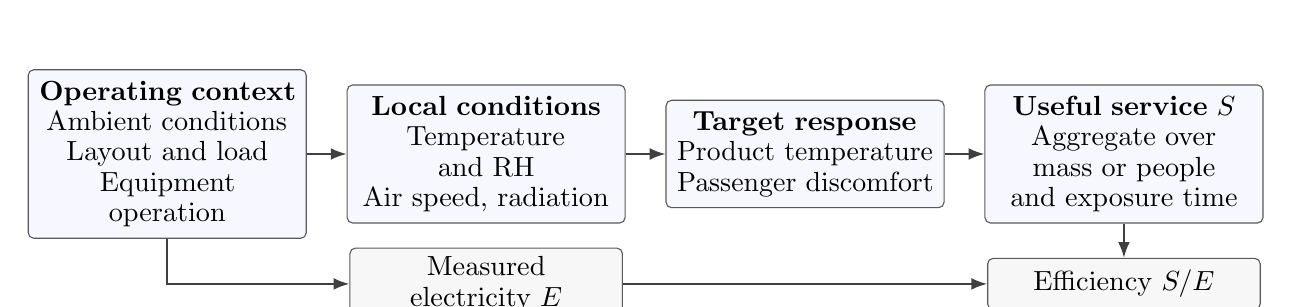
\begin{tikzpicture}[
  font=\fontsize{10}{11}\selectfont,
  stage/.style={draw=black!65,fill=blue!3,rounded corners=2pt,
    text width=3.25cm,minimum height=1.35cm,align=center,inner sep=4pt},
  account/.style={draw=black!65,fill=black!3,rounded corners=2pt,
    text width=3.25cm,minimum height=0.65cm,align=center,inner sep=3pt},
  flow/.style={-{Latex[length=2mm]},line width=0.65pt,draw=black!75}]
\node[stage] (context) at (0,0)
  {\textbf{Operating context}\\Ambient conditions\\Layout and load\\Equipment operation};
\node[stage] (local) at (4.05,0)
  {\textbf{Local conditions}\\Temperature and RH\\Air speed, radiation};
\node[stage] (response) at (8.10,0)
  {\textbf{Target response}\\Product temperature\\Passenger discomfort};
\node[stage] (service) at (12.15,0)
  {\textbf{Useful service} $S$\\Aggregate over\\mass or people\\and exposure time};
\node[account] (energy) at (4.05,-1.65)
  {Measured electricity $E$};
\node[account] (efficiency) at (12.15,-1.65)
  {Efficiency $S/E$};
\draw[flow] (context) -- (local);
\draw[flow] (local) -- (response);
\draw[flow] (response) -- (service);
\draw[flow] (context.south) |- (energy.west);
\draw[flow] (energy.east) -- (efficiency.west);
\draw[flow] (service.south) -- (efficiency.north);
\end{tikzpicture}
\caption{Process linking conditions to service and electricity over the same period ($E>0$).}
\label{fig:process}
\end{figure}

\clearpage
\subsection{Factors that explain performance}

Figure~\ref{fig:process} traces how operating conditions become delivered service. The arrows represent physical dependencies and service accounting; feedback and transient responses are handled within the later models. This process-oriented exposition draws on a supplied AI analysis, with the dependencies revised here \cite{gemini}.

\noindent\textbf{From surroundings to local conditions.} Infiltration carries sensible heat and moisture through the opening; walls transmit heat, and exposed surfaces exchange radiation. Geometry, insulation, ambient temperature, humidity, and airflow therefore alter the conditions around the products and the refrigeration demand \cite{ashrae}.

\noindent\textbf{From operation to local conditions.} Lights and fans release heat, warmer incoming stock adds a temporary load, and defrost interrupts normal cooling \cite{ashrae}. Equipment condition changes insulation, airflow, and power demand. These mechanisms affect both local conditions and measured electricity; age itself is not an additional score.

\noindent\textbf{From local conditions to service.} Product placement and thermal response determine whether the food remains within its required range. Accumulating compliant product mass over time gives useful storage service. The same sequence applies to passengers, but their response depends on the thermal environment and their exposure, rather than food-temperature limits.

\subsection{Implications for the bus-stop model}

The preceding analysis motivates a common evaluation principle:
\begin{equation}
\boxed{\text{Cooling efficiency}
=\frac{\text{useful service accumulated over objects and time}}
{\text{energy input over the same period}}.}
\label{eq:principle}
\end{equation}

The freezer measure can be expressed in compliant kg\,h per kWh. At a bus stop, useful service accumulates thermal-discomfort reduction over people and waiting time. The next model specifies this response and spatial calculation; the two settings do not have numerically comparable units.

First, \textbf{evaluate people directly}. A fan changes local air movement and can improve thermal sensation without lowering air temperature \cite{energystar}. A direct evaporative cooler changes temperature and humidity \cite{evap}. Device-specific mechanisms therefore feed into a common assessment of passenger response.

Second, \textbf{weight effects by occupancy}. Geometry and airflow determine which occupied zones benefit; cooling empty space receives no passenger-service credit. Area is not multiplied by total headcount again. Outdoor air exchange may disperse cooled air while changing local air movement, so its effect is assessed through passenger response.

Third, \textbf{retain a minimum-service check}. Check individual product-temperature excursions and remaining unacceptable passenger exposure even when aggregate service is high. Partial relief can count as a benefit without establishing adequacy; minimum requirements remain separate from the efficiency score.

Within a venue, compare strategies under matched weather, occupancy, geometry, and evaluation periods. Water use, operating cost, and broader visitor experience enter the later effectiveness model. AI-assisted analysis and drafting are recorded in the appended report \cite{codex}.

\clearpage
\section{Cooling a Bus Stop: From Local Conditions to Passenger Service}
\label{sec:bus}

We apply the service principle in Section~\ref{sec:understand} to Requirement 2(a). A device first changes the environment at each passenger's position; those changes alter thermal discomfort; the resulting relief is accumulated over people and time. This separates three questions: how much relief is delivered, where it is delivered, and how much electricity it requires.

\subsection{Data, interpretation, and a reproducible scenario}

The problem describes A as a fan with an apparent cooling effect of up to $3\,^{\circ}\mathrm C$, and B and C as evaporative coolers with air-temperature reductions of up to $5$ and $8\,^{\circ}\mathrm C$ \cite{problem}. These effects use different temperature concepts. We do not subtract $3\,^{\circ}\mathrm C$ from the air temperature for A or treat its unspecified ``feels like'' index as measured SET.

The table labels energy use in kW/hr. To obtain a dimensionally consistent comparison, \textbf{we interpret its numerical entries as mean operating powers} $P_A=0.25$, $P_B=1.2$, and $P_C=2.5$ kW. Thus a one-hour comparison uses $0.25$, $1.2$, and $2.5$ kWh. This is a stated interpretation, not a verified correction to equipment specifications.

The problem supplies no airflow, coverage map, rating weather, or evaporative effectiveness. Therefore, the numerical analysis below is an \textbf{illustrative scenario analysis, not an identification of actual device performance}. Table~\ref{tab:bus-assumptions} specifies the common environment; Table~\ref{tab:bus-fields} specifies the uncertain delivered fields before comparing outcomes.

\begin{table}[!ht]
\centering\small
\caption{Common scenario assumptions, shared by all three devices.}
\label{tab:bus-assumptions}
\renewcommand{\arraystretch}{1.12}
\begin{tabularx}{\linewidth}{@{}p{0.31\linewidth}X@{}}
\toprule
Quantity & Assumed value and meaning\\
\midrule
Shelter & Shaded $6\times2$ m footprint; three equal $4\,\mathrm{m^2}$ near, middle, and edge zones.\\
Weather & $T_a=34\,^{\circ}\mathrm C$; dry/humid cases RH $=30/70\%$; sweep $20$--$80\%$.\\
Radiation and background air & Mean radiant temperature $T_r=36\,^{\circ}\mathrm C$; baseline local speed $v_0=0.20$ m/s; pressure $101325$ Pa.\\
Reference passenger & Standing, $1.2$ met, $0.5$ clo; default body area $1.8258\,\mathrm{m^2}$ and zero external work in the SET implementation.\\
Occupancy and period & Mean simultaneous occupancy $(4,4,4)$ over one hour: $12$ person-hours, not a one-hour wait for every passenger.\\
Alternative distributions & Near-heavy $(8,3,1)$ and edge-heavy $(1,3,8)$; both retain the same total of 12 people.\\
Decision threshold & SET threshold $\Theta_c=26\,^{\circ}\mathrm C$, an assumed hot-discomfort reference; tested at $24$ and $28\,^{\circ}\mathrm C$.\\
\bottomrule
\end{tabularx}
\end{table}

\begin{table}[!ht]
\centering\small
\caption{Assumed local delivery profiles. Entries follow near/middle/edge order.}
\label{tab:bus-fields}
\begin{tabularx}{\linewidth}{@{}lXXc@{}}
\toprule
Device & Local air speed (m/s) & Cooled-air mass fraction $f_{s,z}$ & $\varepsilon_s$\\
\midrule
A & $1.00 / 0.55 / 0.25$ & $0 / 0 / 0$ & ---\\
B & $0.80 / 0.50 / 0.30$ & $0.80 / 0.45 / 0.10$ & $0.70$\\
C & $1.00 / 0.80 / 0.50$ & $0.90 / 0.70 / 0.40$ & $0.70$\\
\bottomrule
\end{tabularx}
\end{table}

Here $f_{s,z}$ is the local dry-air mass mixing fraction of treated air, not a division of the device's total flow among zones; its three entries need not sum to one. The larger coverage assumed for C is tested, not presented as a fact supplied by the problem.

\clearpage
\subsection{Predicting the local environment}

\noindent\textbf{Fan A: air movement.} We set $T_{A,z}=T_a$ and retain ambient moisture, while prescribing local speeds from Table~\ref{tab:bus-fields}. The resulting convection and evaporation enter the passenger-response model. This follows the physical distinction between moving air and lowering dry-bulb temperature \cite{fanguide}. We neglect the fan motor's small local heat plume in this open, mixed-air approximation.

\noindent\textbf{B and C: evaporation followed by dilution.} Direct evaporation reduces dry-bulb temperature while increasing moisture; the entering wet-bulb temperature $T_{wb}$ limits the achievable depression \cite{evapequip}. We adopt
\begin{equation}
 T_{o,s}=T_a-\min\{\Delta T_s^{\max},\;\varepsilon_s(T_a-T_{wb})\},
 \qquad s\in\{B,C\},
\label{eq:outlet}
\end{equation}
where $\Delta T_B^{\max}=5$ and $\Delta T_C^{\max}=8\,^{\circ}\mathrm C$. Applying these advertised shelter-temperature reductions as outlet caps is an explicit modeling convention; the problem does not specify their measurement location. The caps do not imply that either device achieves them under every climate.

Let $w$ denote kg of water vapor per kg of dry air and $h$ the moist-air enthalpy in kJ/kg of dry air. Using standard SI psychrometric relations \cite{psychrolib},
\begin{align}
 w&=0.621945\frac{p_v}{p-p_v},\qquad p_v=\phi p_{sat}(T),\\
 h(T,w)&=1.006T+w(2501+1.86T),
\label{eq:enthalpy}
\end{align}
where $\phi$ is RH as a fraction. Approximating evaporation as isenthalpic, $h_{o,s}\simeq h_a$, gives
\begin{equation}
 w_{o,s}=\frac{h_a-1.006T_{o,s}}{2501+1.86T_{o,s}}.
\end{equation}
This neglects fan heat and make-up-water enthalpy; near-constant enthalpy is not an assertion of exact constant wet-bulb temperature \cite{evap}.

Outdoor dilution is represented by a two-stream balance on dry-air mass:
\begin{align}
 w_{s,z}&=(1-f_{s,z})w_a+f_{s,z}w_{o,s},\\
 h_{s,z}&=(1-f_{s,z})h_a+f_{s,z}h_{o,s},\\
 T_{s,z}&=\frac{h_{s,z}-2501w_{s,z}}{1.006+1.86w_{s,z}}.
\label{eq:mixing}
\end{align}
We recover RH from $T_{s,z}$ and $w_{s,z}$, rather than averaging RH directly. Every calculated state is checked against saturation. This reduced model needs measured local delivery profiles for site-specific predictions; it is not a CFD calculation.

\subsection{Converting local conditions to a common human response}

We compute standard effective temperature (SET), denoted $\Theta$, from
\begin{equation}
 \Theta_{s,z}=F_{\mathrm{SET}}(T_{s,z},T_{r,z},v_{s,z},\phi_{s,z};\mathrm{met},\mathrm{clo}).
\label{eq:set}
\end{equation}
SET compares physiological heat exchange with that in a reference environment, making it more suitable here than air-temperature drop alone \cite{thermalcomfort,fanguide}. We use the published \texttt{pythermalcomfort} implementation with input-domain checks enabled \cite{pythermal}. All scenario inputs remain inside its documented temperature, air-speed, clothing, and activity limits. SET is used as a quasi-steady engineering comparison: its reference conditions originate in typical indoor applications, and it does not model a passenger's prior walking or individual transient response \cite{thermalcomfort}.

\clearpage
\subsection{Measuring service and retaining a quality check}

For the warm-weather scenarios, define the hot-discomfort proxy
\begin{equation}
 D(\Theta)=[\Theta-\Theta_c]_+,\qquad [x]_+=\max(x,0).
\end{equation}
The threshold is a decision assumption, not an ASHRAE safety limit. Let $0$ denote the same shelter without active cooling, retaining the same shade, weather, radiation, and background air movement. The signed local improvement is
\begin{equation}
 b_{s,z,k}=D(\Theta_{0,z,k})-D(\Theta_{s,z,k}).
\end{equation}
Negative values are retained: an adverse condition must reduce useful service. Over time steps of $\Delta t_k$ hours,
\begin{align}
 U_s&=\sum_k\sum_z n_{z,k}b_{s,z,k}\Delta t_k, &
 E_s&=\sum_k P_{s,k}\Delta t_k,\\
 \eta_s&=U_s/E_s,\qquad E_s>0.
\label{eq:bus-efficiency}
\end{align}
The unit of $\eta$ is person$\cdot{}^{\circ}\mathrm C\cdot$h/kWh, with temperature measured on the SET scale. This is a service-efficiency index, not a thermodynamic percentage or COP. Empty zones earn no credit, although operating electricity is still counted. The zero-energy baseline has no efficiency ratio.

We also report remaining discomfort,
\begin{equation}
 R_s=\sum_k\sum_z n_{z,k}D(\Theta_{s,z,k})\Delta t_k,
 \qquad \overline D_s=\frac{R_s}{\sum_k\sum_z n_{z,k}\Delta t_k}.
\label{eq:remaining}
\end{equation}
A high $\eta_s$ alone does not establish adequate relief. If a decision-maker specifies an acceptable residual or an individual exposure requirement, it should be imposed separately; no universal heat-health threshold is inferred from our SET proxy. When the baseline already meets the chosen hot-discomfort criterion, further cooling earns no benefit, and switching off can be appropriate.

\noindent\textbf{Why area and population do not become extra multipliers.} If $n_z=\rho_zA_z$, footprint and population are already represented. Multiplying $U_s$ by shelter area or total headcount again would count the same service twice. Increasing every $n_z$ by a common factor scales every $\eta_s$ equally and cannot change ranking unless spatial distribution or delivered conditions also change.

\noindent\textbf{A ranking result independent of the assumed delivery maps.} Under the interpreted constant powers and a common operating period,
\begin{align}
 \eta_B>\eta_A&\iff U_B>4.8U_A,\nonumber\\
 \eta_C>\eta_A&\iff U_C>10U_A,\\
 \eta_C>\eta_B&\iff U_C>\frac{25}{12}U_B.\nonumber
\label{eq:break-even}
\end{align}
Thus nominal temperature reduction alone cannot justify a larger device. Its accumulated passenger relief must compensate for its larger electricity input. These inequalities follow from the given power ratios; their validity does not depend on the assumed zone profiles.

\clearpage
\subsection{Numerical results: local mechanisms and the efficiency tradeoff}

\begin{figure}[!ht]
\centering
% Self-contained Figure 1. Source: local_conditions.csv, Uniform occupancy.
% RGB values reproduce the PNG colormaps; each column shares one scale across climates.
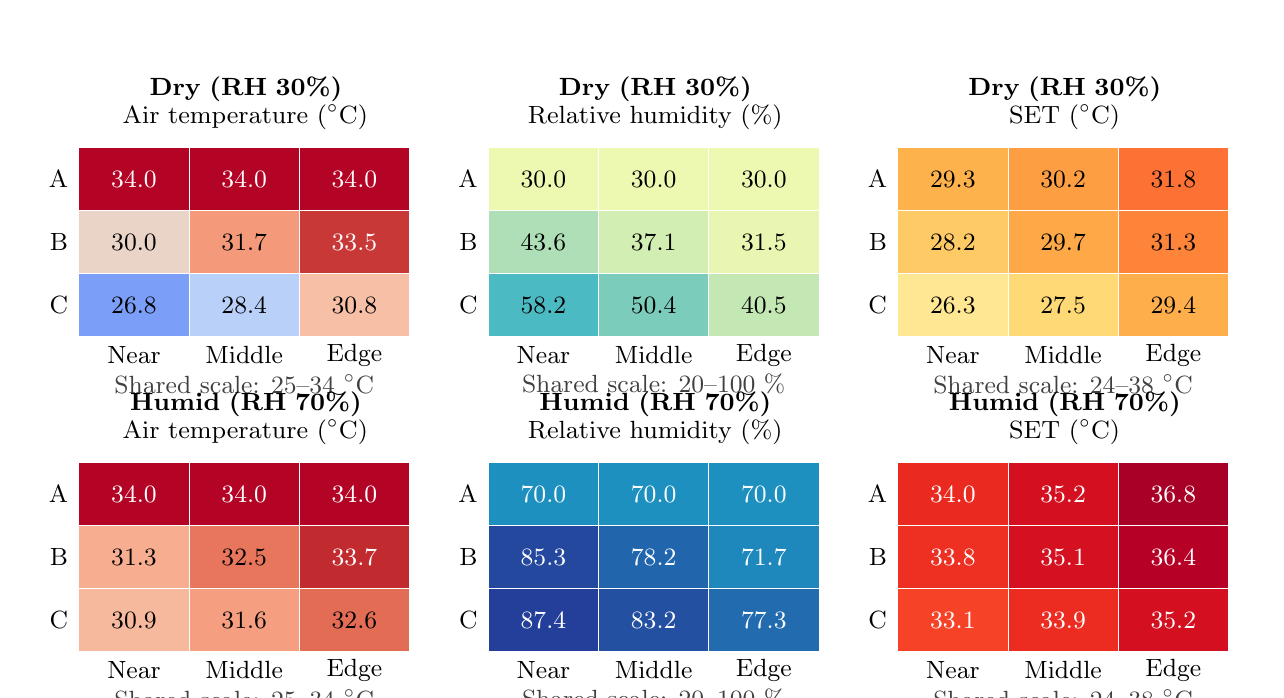
\begin{tikzpicture}[x=1cm,y=1cm,every node/.style={font=\fontsize{9}{10}\selectfont,inner sep=0pt}]
\path[use as bounding box] (0,0) rectangle (15.6,8.15);
\node[align=center,text width=4.9cm] at (2.750,7.720) {\textbf{Dry (RH 30\%)}\\Air temperature ($^{\circ}$C)};
\node[anchor=east] at (0.520,6.750) {A};
\definecolor{busLocal0000}{rgb}{0.705673,0.015556,0.150233}
\filldraw[fill=busLocal0000,draw=white,line width=0.35pt] (0.650,6.350) rectangle (2.050,7.150);
\node[text=white] at (1.350,6.750) {34.0};
\definecolor{busLocal0001}{rgb}{0.705673,0.015556,0.150233}
\filldraw[fill=busLocal0001,draw=white,line width=0.35pt] (2.050,6.350) rectangle (3.450,7.150);
\node[text=white] at (2.750,6.750) {34.0};
\definecolor{busLocal0002}{rgb}{0.705673,0.015556,0.150233}
\filldraw[fill=busLocal0002,draw=white,line width=0.35pt] (3.450,6.350) rectangle (4.850,7.150);
\node[text=white] at (4.150,6.750) {34.0};
\node[anchor=east] at (0.520,5.950) {B};
\definecolor{busLocal0010}{rgb}{0.919376,0.831273,0.782874}
\filldraw[fill=busLocal0010,draw=white,line width=0.35pt] (0.650,5.550) rectangle (2.050,6.350);
\node[text=black] at (1.350,5.950) {30.0};
\definecolor{busLocal0011}{rgb}{0.958279,0.604335,0.483297}
\filldraw[fill=busLocal0011,draw=white,line width=0.35pt] (2.050,5.550) rectangle (3.450,6.350);
\node[text=black] at (2.750,5.950) {31.7};
\definecolor{busLocal0012}{rgb}{0.785153,0.220851,0.211673}
\filldraw[fill=busLocal0012,draw=white,line width=0.35pt] (3.450,5.550) rectangle (4.850,6.350);
\node[text=white] at (4.150,5.950) {33.5};
\node[anchor=east] at (0.520,5.150) {C};
\definecolor{busLocal0020}{rgb}{0.483854,0.622050,0.974808}
\filldraw[fill=busLocal0020,draw=white,line width=0.35pt] (0.650,4.750) rectangle (2.050,5.550);
\node[text=black] at (1.350,5.150) {26.8};
\definecolor{busLocal0021}{rgb}{0.724041,0.814910,0.975651}
\filldraw[fill=busLocal0021,draw=white,line width=0.35pt] (2.050,4.750) rectangle (3.450,5.550);
\node[text=black] at (2.750,5.150) {28.4};
\definecolor{busLocal0022}{rgb}{0.963772,0.749086,0.649420}
\filldraw[fill=busLocal0022,draw=white,line width=0.35pt] (3.450,4.750) rectangle (4.850,5.550);
\node[text=black] at (4.150,5.150) {30.8};
\node at (1.350,4.520) {Near};
\node at (2.750,4.520) {Middle};
\node at (4.150,4.520) {Edge};
\node[text=black!75] at (2.750,4.150) {Shared scale: 25--34 $^{\circ}$C};
\node[align=center,text width=4.9cm] at (7.950,7.720) {\textbf{Dry (RH 30\%)}\\Relative humidity (\%)};
\node[anchor=east] at (5.720,6.750) {A};
\definecolor{busLocal0100}{rgb}{0.928827,0.972318,0.694164}
\filldraw[fill=busLocal0100,draw=white,line width=0.35pt] (5.850,6.350) rectangle (7.250,7.150);
\node[text=black] at (6.550,6.750) {30.0};
\definecolor{busLocal0101}{rgb}{0.928827,0.972318,0.694164}
\filldraw[fill=busLocal0101,draw=white,line width=0.35pt] (7.250,6.350) rectangle (8.650,7.150);
\node[text=black] at (7.950,6.750) {30.0};
\definecolor{busLocal0102}{rgb}{0.928827,0.972318,0.694164}
\filldraw[fill=busLocal0102,draw=white,line width=0.35pt] (8.650,6.350) rectangle (10.050,7.150);
\node[text=black] at (9.350,6.750) {30.0};
\node[anchor=east] at (5.720,5.950) {B};
\definecolor{busLocal0110}{rgb}{0.680738,0.874971,0.715571}
\filldraw[fill=busLocal0110,draw=white,line width=0.35pt] (5.850,5.550) rectangle (7.250,6.350);
\node[text=black] at (6.550,5.950) {43.6};
\definecolor{busLocal0111}{rgb}{0.825975,0.931719,0.702284}
\filldraw[fill=busLocal0111,draw=white,line width=0.35pt] (7.250,5.550) rectangle (8.650,6.350);
\node[text=black] at (7.950,5.950) {37.1};
\definecolor{busLocal0112}{rgb}{0.910127,0.964937,0.695640}
\filldraw[fill=busLocal0112,draw=white,line width=0.35pt] (8.650,5.550) rectangle (10.050,6.350);
\node[text=black] at (9.350,5.950) {31.5};
\node[anchor=east] at (5.720,5.150) {C};
\definecolor{busLocal0120}{rgb}{0.296855,0.729289,0.762537}
\filldraw[fill=busLocal0120,draw=white,line width=0.35pt] (5.850,4.750) rectangle (7.250,5.550);
\node[text=black] at (6.550,5.150) {58.2};
\definecolor{busLocal0121}{rgb}{0.487551,0.800031,0.734856}
\filldraw[fill=busLocal0121,draw=white,line width=0.35pt] (7.250,4.750) rectangle (8.650,5.550);
\node[text=black] at (7.950,5.150) {50.4};
\definecolor{busLocal0122}{rgb}{0.769319,0.909419,0.706959}
\filldraw[fill=busLocal0122,draw=white,line width=0.35pt] (8.650,4.750) rectangle (10.050,5.550);
\node[text=black] at (9.350,5.150) {40.5};
\node at (6.550,4.520) {Near};
\node at (7.950,4.520) {Middle};
\node at (9.350,4.520) {Edge};
\node[text=black!75] at (7.950,4.150) {Shared scale: 20--100 \%};
\node[align=center,text width=4.9cm] at (13.150,7.720) {\textbf{Dry (RH 30\%)}\\SET ($^{\circ}$C)};
\node[anchor=east] at (10.920,6.750) {A};
\definecolor{busLocal0200}{rgb}{0.996032,0.696332,0.297301}
\filldraw[fill=busLocal0200,draw=white,line width=0.35pt] (11.050,6.350) rectangle (12.450,7.150);
\node[text=black] at (11.750,6.750) {29.3};
\definecolor{busLocal0201}{rgb}{0.993941,0.618947,0.263837}
\filldraw[fill=busLocal0201,draw=white,line width=0.35pt] (12.450,6.350) rectangle (13.850,7.150);
\node[text=black] at (13.150,6.750) {30.2};
\definecolor{busLocal0202}{rgb}{0.990496,0.448304,0.205398}
\filldraw[fill=busLocal0202,draw=white,line width=0.35pt] (13.850,6.350) rectangle (15.250,7.150);
\node[text=black] at (14.550,6.750) {31.8};
\node[anchor=east] at (10.920,5.950) {B};
\definecolor{busLocal0210}{rgb}{0.996078,0.792203,0.399446}
\filldraw[fill=busLocal0210,draw=white,line width=0.35pt] (11.050,5.550) rectangle (12.450,6.350);
\node[text=black] at (11.750,5.950) {28.2};
\definecolor{busLocal0211}{rgb}{0.995048,0.659915,0.281553}
\filldraw[fill=busLocal0211,draw=white,line width=0.35pt] (12.450,5.550) rectangle (13.850,6.350);
\node[text=black] at (13.150,5.950) {29.7};
\definecolor{busLocal0212}{rgb}{0.991603,0.518062,0.225329}
\filldraw[fill=busLocal0212,draw=white,line width=0.35pt] (13.850,5.550) rectangle (15.250,6.350);
\node[text=black] at (14.550,5.950) {31.3};
\node[anchor=east] at (10.920,5.150) {C};
\definecolor{busLocal0220}{rgb}{0.998754,0.904498,0.575133}
\filldraw[fill=busLocal0220,draw=white,line width=0.35pt] (11.050,4.750) rectangle (12.450,5.550);
\node[text=black] at (11.750,5.150) {26.3};
\definecolor{busLocal0221}{rgb}{0.996078,0.849781,0.461453}
\filldraw[fill=busLocal0221,draw=white,line width=0.35pt] (12.450,4.750) rectangle (13.850,5.550);
\node[text=black] at (13.150,5.150) {27.5};
\definecolor{busLocal0222}{rgb}{0.995663,0.682676,0.291396}
\filldraw[fill=busLocal0222,draw=white,line width=0.35pt] (13.850,4.750) rectangle (15.250,5.550);
\node[text=black] at (14.550,5.150) {29.4};
\node at (11.750,4.520) {Near};
\node at (13.150,4.520) {Middle};
\node at (14.550,4.520) {Edge};
\node[text=black!75] at (13.150,4.150) {Shared scale: 24--38 $^{\circ}$C};
\node[align=center,text width=4.9cm] at (2.750,3.720) {\textbf{Humid (RH 70\%)}\\Air temperature ($^{\circ}$C)};
\node[anchor=east] at (0.520,2.750) {A};
\definecolor{busLocal1000}{rgb}{0.705673,0.015556,0.150233}
\filldraw[fill=busLocal1000,draw=white,line width=0.35pt] (0.650,2.350) rectangle (2.050,3.150);
\node[text=white] at (1.350,2.750) {34.0};
\definecolor{busLocal1001}{rgb}{0.705673,0.015556,0.150233}
\filldraw[fill=busLocal1001,draw=white,line width=0.35pt] (2.050,2.350) rectangle (3.450,3.150);
\node[text=white] at (2.750,2.750) {34.0};
\definecolor{busLocal1002}{rgb}{0.705673,0.015556,0.150233}
\filldraw[fill=busLocal1002,draw=white,line width=0.35pt] (3.450,2.350) rectangle (4.850,3.150);
\node[text=white] at (4.150,2.750) {34.0};
\node[anchor=east] at (0.520,1.950) {B};
\definecolor{busLocal1010}{rgb}{0.968894,0.679480,0.562812}
\filldraw[fill=busLocal1010,draw=white,line width=0.35pt] (0.650,1.550) rectangle (2.050,2.350);
\node[text=black] at (1.350,1.950) {31.3};
\definecolor{busLocal1011}{rgb}{0.908908,0.462433,0.360950}
\filldraw[fill=busLocal1011,draw=white,line width=0.35pt] (2.050,1.550) rectangle (3.450,2.350);
\node[text=black] at (2.750,1.950) {32.5};
\definecolor{busLocal1012}{rgb}{0.758112,0.168122,0.188827}
\filldraw[fill=busLocal1012,draw=white,line width=0.35pt] (3.450,1.550) rectangle (4.850,2.350);
\node[text=white] at (4.150,1.950) {33.7};
\node[anchor=east] at (0.520,1.150) {C};
\definecolor{busLocal1020}{rgb}{0.967874,0.725847,0.618489}
\filldraw[fill=busLocal1020,draw=white,line width=0.35pt] (0.650,0.750) rectangle (2.050,1.550);
\node[text=black] at (1.350,1.150) {30.9};
\definecolor{busLocal1021}{rgb}{0.961595,0.622247,0.501551}
\filldraw[fill=busLocal1021,draw=white,line width=0.35pt] (2.050,0.750) rectangle (3.450,1.550);
\node[text=black] at (2.750,1.150) {31.6};
\definecolor{busLocal1022}{rgb}{0.892138,0.425389,0.333289}
\filldraw[fill=busLocal1022,draw=white,line width=0.35pt] (3.450,0.750) rectangle (4.850,1.550);
\node[text=black] at (4.150,1.150) {32.6};
\node at (1.350,0.520) {Near};
\node at (2.750,0.520) {Middle};
\node at (4.150,0.520) {Edge};
\node[text=black!75] at (2.750,0.150) {Shared scale: 25--34 $^{\circ}$C};
\node[align=center,text width=4.9cm] at (7.950,3.720) {\textbf{Humid (RH 70\%)}\\Relative humidity (\%)};
\node[anchor=east] at (5.720,2.750) {A};
\definecolor{busLocal1100}{rgb}{0.114110,0.564706,0.751096}
\filldraw[fill=busLocal1100,draw=white,line width=0.35pt] (5.850,2.350) rectangle (7.250,3.150);
\node[text=white] at (6.550,2.750) {70.0};
\definecolor{busLocal1101}{rgb}{0.114110,0.564706,0.751096}
\filldraw[fill=busLocal1101,draw=white,line width=0.35pt] (7.250,2.350) rectangle (8.650,3.150);
\node[text=white] at (7.950,2.750) {70.0};
\definecolor{busLocal1102}{rgb}{0.114110,0.564706,0.751096}
\filldraw[fill=busLocal1102,draw=white,line width=0.35pt] (8.650,2.350) rectangle (10.050,3.150);
\node[text=white] at (9.350,2.750) {70.0};
\node[anchor=east] at (5.720,1.950) {B};
\definecolor{busLocal1110}{rgb}{0.139516,0.282076,0.617609}
\filldraw[fill=busLocal1110,draw=white,line width=0.35pt] (5.850,1.550) rectangle (7.250,2.350);
\node[text=white] at (6.550,1.950) {85.3};
\definecolor{busLocal1111}{rgb}{0.130104,0.401569,0.674325}
\filldraw[fill=busLocal1111,draw=white,line width=0.35pt] (7.250,1.550) rectangle (8.650,2.350);
\node[text=white] at (7.950,1.950) {78.2};
\definecolor{busLocal1112}{rgb}{0.117186,0.533333,0.736332}
\filldraw[fill=busLocal1112,draw=white,line width=0.35pt] (8.650,1.550) rectangle (10.050,2.350);
\node[text=white] at (9.350,1.950) {71.7};
\node[anchor=east] at (5.720,1.150) {C};
\definecolor{busLocal1120}{rgb}{0.142099,0.245905,0.600384}
\filldraw[fill=busLocal1120,draw=white,line width=0.35pt] (5.850,0.750) rectangle (7.250,1.550);
\node[text=white] at (6.550,1.150) {87.4};
\definecolor{busLocal1121}{rgb}{0.137301,0.313080,0.632372}
\filldraw[fill=busLocal1121,draw=white,line width=0.35pt] (7.250,0.750) rectangle (8.650,1.550);
\node[text=white] at (7.950,1.150) {83.2};
\definecolor{busLocal1122}{rgb}{0.128258,0.420392,0.683183}
\filldraw[fill=busLocal1122,draw=white,line width=0.35pt] (8.650,0.750) rectangle (10.050,1.550);
\node[text=white] at (9.350,1.150) {77.3};
\node at (6.550,0.520) {Near};
\node at (7.950,0.520) {Middle};
\node at (9.350,0.520) {Edge};
\node[text=black!75] at (7.950,0.150) {Shared scale: 20--100 \%};
\node[align=center,text width=4.9cm] at (13.150,3.720) {\textbf{Humid (RH 70\%)}\\SET ($^{\circ}$C)};
\node[anchor=east] at (10.920,2.750) {A};
\definecolor{busLocal1200}{rgb}{0.918647,0.161138,0.125736}
\filldraw[fill=busLocal1200,draw=white,line width=0.35pt] (11.050,2.350) rectangle (12.450,3.150);
\node[text=white] at (11.750,2.750) {34.0};
\definecolor{busLocal1201}{rgb}{0.830588,0.061176,0.125490}
\filldraw[fill=busLocal1201,draw=white,line width=0.35pt] (12.450,2.350) rectangle (13.850,3.150);
\node[text=white] at (13.150,2.750) {35.2};
\definecolor{busLocal1202}{rgb}{0.659562,0.000000,0.149020}
\filldraw[fill=busLocal1202,draw=white,line width=0.35pt] (13.850,2.350) rectangle (15.250,3.150);
\node[text=white] at (14.550,2.750) {36.8};
\node[anchor=east] at (10.920,1.950) {B};
\definecolor{busLocal1210}{rgb}{0.930950,0.186728,0.132626}
\filldraw[fill=busLocal1210,draw=white,line width=0.35pt] (11.050,1.550) rectangle (12.450,2.350);
\node[text=white] at (11.750,1.950) {33.8};
\definecolor{busLocal1211}{rgb}{0.835263,0.064375,0.124260}
\filldraw[fill=busLocal1211,draw=white,line width=0.35pt] (12.450,1.550) rectangle (13.850,2.350);
\node[text=white] at (13.150,1.950) {35.1};
\definecolor{busLocal1212}{rgb}{0.719600,0.000000,0.149020}
\filldraw[fill=busLocal1212,draw=white,line width=0.35pt] (13.850,1.550) rectangle (15.250,2.350);
\node[text=white] at (14.550,1.950) {36.4};
\node[anchor=east] at (10.920,1.150) {C};
\definecolor{busLocal1220}{rgb}{0.964783,0.257101,0.151572}
\filldraw[fill=busLocal1220,draw=white,line width=0.35pt] (11.050,0.750) rectangle (12.450,1.550);
\node[text=white] at (11.750,1.150) {33.1};
\definecolor{busLocal1221}{rgb}{0.924798,0.173933,0.129181}
\filldraw[fill=busLocal1221,draw=white,line width=0.35pt] (12.450,0.750) rectangle (13.850,1.550);
\node[text=white] at (13.150,1.150) {33.9};
\definecolor{busLocal1222}{rgb}{0.830588,0.061176,0.125490}
\filldraw[fill=busLocal1222,draw=white,line width=0.35pt] (13.850,0.750) rectangle (15.250,1.550);
\node[text=white] at (14.550,1.150) {35.2};
\node at (11.750,0.520) {Near};
\node at (13.150,0.520) {Middle};
\node at (14.550,0.520) {Edge};
\node[text=black!75] at (13.150,0.150) {Shared scale: 24--38 $^{\circ}$C};
\end{tikzpicture}

\caption{Simulated local air temperature, RH, and SET under the stated assumptions. Fan A leaves air temperature unchanged while changing SET. B and C lower air temperature and increase RH. These are scenario outputs, not field measurements.}
\label{fig:bus-local}
\end{figure}

Spatial delivery matters even within one small shelter. In the dry case, C gives SET $26.3\,^{\circ}\mathrm C$ near the outlet but $29.4\,^{\circ}\mathrm C$ at the edge. At RH $70\%$, these become $33.1$ and $35.2\,^{\circ}\mathrm C$. A single mean air-temperature reduction would conceal these differences. A, meanwhile, improves SET without changing the $34\,^{\circ}\mathrm C$ dry-bulb temperature.

\begin{figure}[!ht]
\centering
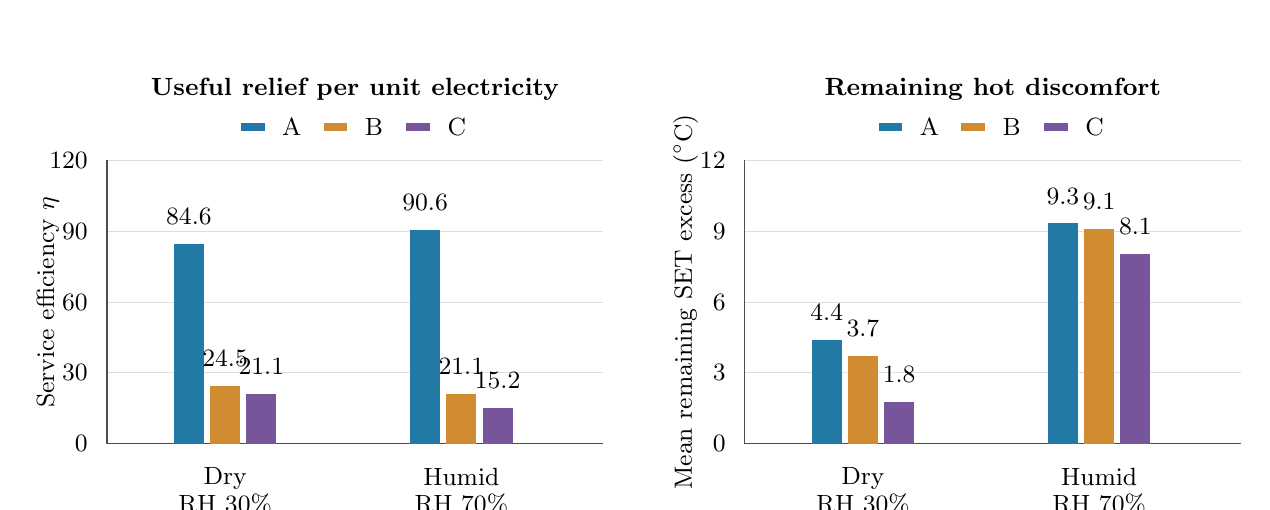
\begin{tikzpicture}[x=1cm,y=1cm,font=\fontsize{9}{10}\selectfont]
\definecolor{busA}{HTML}{2379A5}
\definecolor{busB}{HTML}{D18C32}
\definecolor{busC}{HTML}{76559A}
\begin{scope}[xshift=0.0cm]
\draw[black!13] (0.0000,0.0000) -- (6.3000,0.0000);
\node[anchor=east] at (-0.1200,0.0000) {0};
\draw[black!13] (0.0000,0.9000) -- (6.3000,0.9000);
\node[anchor=east] at (-0.1200,0.9000) {30};
\draw[black!13] (0.0000,1.8000) -- (6.3000,1.8000);
\node[anchor=east] at (-0.1200,1.8000) {60};
\draw[black!13] (0.0000,2.7000) -- (6.3000,2.7000);
\node[anchor=east] at (-0.1200,2.7000) {90};
\draw[black!13] (0.0000,3.6000) -- (6.3000,3.6000);
\node[anchor=east] at (-0.1200,3.6000) {120};
\draw[black!70] (0.0000,0.0000) -- (6.3000,0.0000);
\draw[black!70] (0.0000,0.0000) -- (0.0000,3.6000);
\node[align=center] at (3.1500,4.5000) {\textbf{Useful relief per unit electricity}};
\node[rotate=90,align=center] at (-0.7500,1.8000) {Service efficiency $\eta$};
\draw[busA,line width=3pt] (1.7000,4.0200) -- (2.0000,4.0200);
\node[anchor=west] at (2.1000,4.0200) {A};
\draw[busB,line width=3pt] (2.7500,4.0200) -- (3.0500,4.0200);
\node[anchor=west] at (3.1500,4.0200) {B};
\draw[busC,line width=3pt] (3.8000,4.0200) -- (4.1000,4.0200);
\node[anchor=west] at (4.2000,4.0200) {C};
\fill[busA] (0.8500,0) rectangle (1.2300,2.5373);
\node[anchor=south] at (1.0400,2.6573) {84.6};
\fill[busB] (1.3100,0) rectangle (1.6900,0.7353);
\node[anchor=south] at (1.5000,0.8553) {24.5};
\fill[busC] (1.7700,0) rectangle (2.1500,0.6341);
\node[anchor=south] at (1.9600,0.7541) {21.1};
\node[align=center,anchor=north] at (1.5000,-0.1800) {Dry\\RH 30\%};
\fill[busA] (3.8500,0) rectangle (4.2300,2.7171);
\node[anchor=south] at (4.0400,2.8371) {90.6};
\fill[busB] (4.3100,0) rectangle (4.6900,0.6335);
\node[anchor=south] at (4.5000,0.7535) {21.1};
\fill[busC] (4.7700,0) rectangle (5.1500,0.4551);
\node[anchor=south] at (4.9600,0.5751) {15.2};
\node[align=center,anchor=north] at (4.5000,-0.1800) {Humid\\RH 70\%};
\end{scope}
\begin{scope}[xshift=8.1cm]
\draw[black!13] (0.0000,0.0000) -- (6.3000,0.0000);
\node[anchor=east] at (-0.1200,0.0000) {0};
\draw[black!13] (0.0000,0.9000) -- (6.3000,0.9000);
\node[anchor=east] at (-0.1200,0.9000) {3};
\draw[black!13] (0.0000,1.8000) -- (6.3000,1.8000);
\node[anchor=east] at (-0.1200,1.8000) {6};
\draw[black!13] (0.0000,2.7000) -- (6.3000,2.7000);
\node[anchor=east] at (-0.1200,2.7000) {9};
\draw[black!13] (0.0000,3.6000) -- (6.3000,3.6000);
\node[anchor=east] at (-0.1200,3.6000) {12};
\draw[black!70] (0.0000,0.0000) -- (6.3000,0.0000);
\draw[black!70] (0.0000,0.0000) -- (0.0000,3.6000);
\node[align=center] at (3.1500,4.5000) {\textbf{Remaining hot discomfort}};
\node[rotate=90,align=center] at (-0.7500,1.8000) {Mean remaining SET excess ($^{\circ}$C)};
\draw[busA,line width=3pt] (1.7000,4.0200) -- (2.0000,4.0200);
\node[anchor=west] at (2.1000,4.0200) {A};
\draw[busB,line width=3pt] (2.7500,4.0200) -- (3.0500,4.0200);
\node[anchor=west] at (3.1500,4.0200) {B};
\draw[busC,line width=3pt] (3.8000,4.0200) -- (4.1000,4.0200);
\node[anchor=west] at (4.2000,4.0200) {C};
\fill[busA] (0.8500,0) rectangle (1.2300,1.3214);
\node[anchor=south] at (1.0400,1.4414) {4.4};
\fill[busB] (1.3100,0) rectangle (1.6900,1.1147);
\node[anchor=south] at (1.5000,1.2347) {3.7};
\fill[busC] (1.7700,0) rectangle (2.1500,0.5289);
\node[anchor=south] at (1.9600,0.6489) {1.8};
\node[align=center,anchor=north] at (1.5000,-0.1800) {Dry\\RH 30\%};
\fill[busA] (3.8500,0) rectangle (4.2300,2.7981);
\node[anchor=south] at (4.0400,2.9181) {9.3};
\fill[busB] (4.3100,0) rectangle (4.6900,2.7307);
\node[anchor=south] at (4.5000,2.8507) {9.1};
\fill[busC] (4.7700,0) rectangle (5.1500,2.4161);
\node[anchor=south] at (4.9600,2.5361) {8.1};
\node[align=center,anchor=north] at (4.5000,-0.1800) {Humid\\RH 70\%};
\end{scope}
\end{tikzpicture}

\caption{Uniform occupancy: electricity-normalized relief and remaining hot-discomfort proxy. Lower residual is better, whereas higher service efficiency is better. The $26\,^{\circ}\mathrm C$ SET reference is assumed.}
\label{fig:bus-quality}
\end{figure}

For uniform occupancy, dry-case efficiencies are $84.6$, $24.5$, and $21.1$ for A, B, and C, respectively. Yet their mean remaining SET excesses are $4.40$, $3.72$, and $1.76\,^{\circ}\mathrm C$: C delivers more total relief while A delivers more per kWh. At RH $70\%$, efficiencies are $90.6$, $21.1$, and $15.2$; even C retains a mean excess of $8.05\,^{\circ}\mathrm C$. The efficiency winner therefore does not establish that the shelter meets a comfort or safety requirement.

\clearpage
\subsection{Climate and passenger distribution}

\begin{figure}[!ht]
\centering
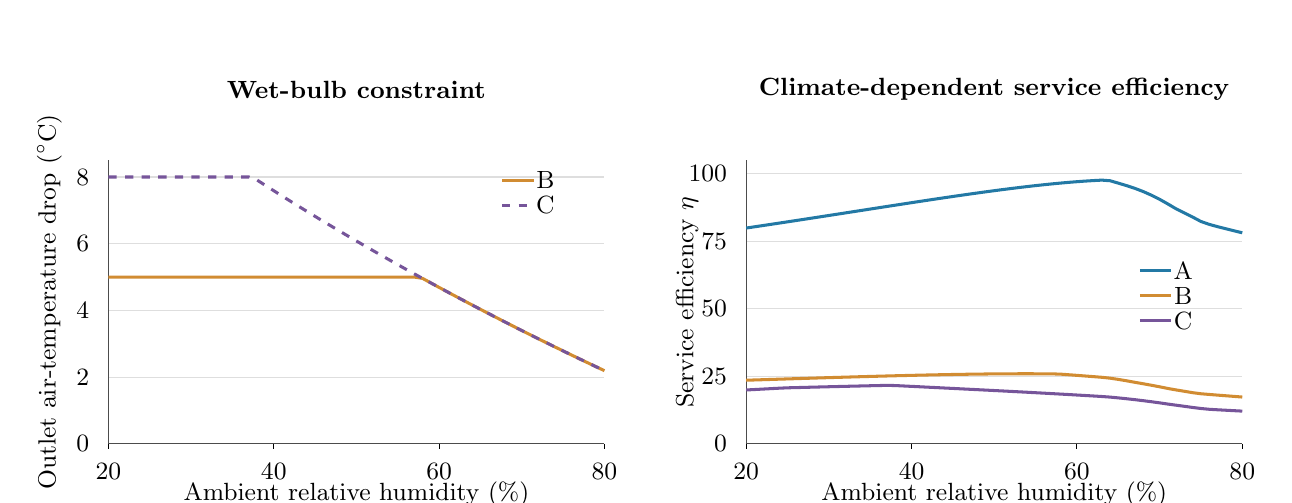
\begin{tikzpicture}[x=1cm,y=1cm,font=\fontsize{9}{10}\selectfont]
\definecolor{busA}{HTML}{2379A5}
\definecolor{busB}{HTML}{D18C32}
\definecolor{busC}{HTML}{76559A}
\begin{scope}[xshift=0.0cm]
\draw[black!13] (0.0000,0.0000) -- (6.3000,0.0000);
\node[anchor=east] at (-0.1200,0.0000) {0};
\draw[black!13] (0.0000,0.8471) -- (6.3000,0.8471);
\node[anchor=east] at (-0.1200,0.8471) {2};
\draw[black!13] (0.0000,1.6941) -- (6.3000,1.6941);
\node[anchor=east] at (-0.1200,1.6941) {4};
\draw[black!13] (0.0000,2.5412) -- (6.3000,2.5412);
\node[anchor=east] at (-0.1200,2.5412) {6};
\draw[black!13] (0.0000,3.3882) -- (6.3000,3.3882);
\node[anchor=east] at (-0.1200,3.3882) {8};
\draw[black!70] (0.0000,0.0000) -- (6.3000,0.0000);
\draw[black!70] (0.0000,0.0000) -- (0.0000,3.6000);
\node[align=center] at (3.1500,4.5000) {\textbf{Wet-bulb constraint}};
\node[rotate=90,align=center] at (-0.7500,1.8000) {Outlet air-temperature drop ($^{\circ}$C)};
\draw[] (0.0000,0.0000) -- (0.0000,-0.0600);
\node[anchor=north] at (0.0000,-0.1300) {20};
\draw[] (2.1000,0.0000) -- (2.1000,-0.0600);
\node[anchor=north] at (2.1000,-0.1300) {40};
\draw[] (4.2000,0.0000) -- (4.2000,-0.0600);
\node[anchor=north] at (4.2000,-0.1300) {60};
\draw[] (6.3000,0.0000) -- (6.3000,-0.0600);
\node[anchor=north] at (6.3000,-0.1300) {80};
\node[] at (3.1500,-0.6400) {Ambient relative humidity (\%)};
\draw[busB,line width=1.1pt] (0.0000,2.1176) -- (0.1050,2.1176) -- (0.2100,2.1176) -- (0.3150,2.1176) -- (0.4200,2.1176) -- (0.5250,2.1176) -- (0.6300,2.1176) -- (0.7350,2.1176) -- (0.8400,2.1176) -- (0.9450,2.1176) -- (1.0500,2.1176) -- (1.1550,2.1176) -- (1.2600,2.1176) -- (1.3650,2.1176) -- (1.4700,2.1176) -- (1.5750,2.1176) -- (1.6800,2.1176) -- (1.7850,2.1176) -- (1.8900,2.1176) -- (1.9950,2.1176) -- (2.1000,2.1176) -- (2.2050,2.1176) -- (2.3100,2.1176) -- (2.4150,2.1176) -- (2.5200,2.1176) -- (2.6250,2.1176) -- (2.7300,2.1176) -- (2.8350,2.1176) -- (2.9400,2.1176) -- (3.0450,2.1176) -- (3.1500,2.1176) -- (3.2550,2.1176) -- (3.3600,2.1176) -- (3.4650,2.1176) -- (3.5700,2.1176) -- (3.6750,2.1176) -- (3.7800,2.1176) -- (3.8850,2.1176) -- (3.9900,2.1005) -- (4.0950,2.0432) -- (4.2000,1.9862) -- (4.3050,1.9297) -- (4.4100,1.8736) -- (4.5150,1.8179) -- (4.6200,1.7625) -- (4.7250,1.7076) -- (4.8300,1.6532) -- (4.9350,1.5990) -- (5.0400,1.5452) -- (5.1450,1.4919) -- (5.2500,1.4390) -- (5.3550,1.3863) -- (5.4600,1.3340) -- (5.5650,1.2821) -- (5.6700,1.2307) -- (5.7750,1.1794) -- (5.8800,1.1285) -- (5.9850,1.0780) -- (6.0900,1.0277) -- (6.1950,0.9780) -- (6.3000,0.9285);
\draw[busC,line width=1.1pt,dashed] (0.0000,3.3882) -- (0.1050,3.3882) -- (0.2100,3.3882) -- (0.3150,3.3882) -- (0.4200,3.3882) -- (0.5250,3.3882) -- (0.6300,3.3882) -- (0.7350,3.3882) -- (0.8400,3.3882) -- (0.9450,3.3882) -- (1.0500,3.3882) -- (1.1550,3.3882) -- (1.2600,3.3882) -- (1.3650,3.3882) -- (1.4700,3.3882) -- (1.5750,3.3882) -- (1.6800,3.3882) -- (1.7850,3.3882) -- (1.8900,3.3484) -- (1.9950,3.2811) -- (2.1000,3.2141) -- (2.2050,3.1479) -- (2.3100,3.0821) -- (2.4150,3.0169) -- (2.5200,2.9524) -- (2.6250,2.8884) -- (2.7300,2.8248) -- (2.8350,2.7617) -- (2.9400,2.6991) -- (3.0450,2.6371) -- (3.1500,2.5756) -- (3.2550,2.5146) -- (3.3600,2.4542) -- (3.4650,2.3941) -- (3.5700,2.3345) -- (3.6750,2.2753) -- (3.7800,2.2166) -- (3.8850,2.1583) -- (3.9900,2.1005) -- (4.0950,2.0432) -- (4.2000,1.9862) -- (4.3050,1.9297) -- (4.4100,1.8736) -- (4.5150,1.8179) -- (4.6200,1.7625) -- (4.7250,1.7076) -- (4.8300,1.6532) -- (4.9350,1.5990) -- (5.0400,1.5452) -- (5.1450,1.4919) -- (5.2500,1.4390) -- (5.3550,1.3863) -- (5.4600,1.3340) -- (5.5650,1.2821) -- (5.6700,1.2307) -- (5.7750,1.1794) -- (5.8800,1.1285) -- (5.9850,1.0780) -- (6.0900,1.0277) -- (6.1950,0.9780) -- (6.3000,0.9285);
\draw[busB,line width=1.1pt] (5.0000,3.3500) -- (5.4000,3.3500);
\node[] at (5.5500,3.3500) {B};
\draw[busC,line width=1.1pt,dashed] (5.0000,3.0300) -- (5.4000,3.0300);
\node[] at (5.5500,3.0300) {C};
\end{scope}
\begin{scope}[xshift=8.1cm]
\draw[black!13] (0.0000,0.0000) -- (6.3000,0.0000);
\node[anchor=east] at (-0.1200,0.0000) {0};
\draw[black!13] (0.0000,0.8571) -- (6.3000,0.8571);
\node[anchor=east] at (-0.1200,0.8571) {25};
\draw[black!13] (0.0000,1.7143) -- (6.3000,1.7143);
\node[anchor=east] at (-0.1200,1.7143) {50};
\draw[black!13] (0.0000,2.5714) -- (6.3000,2.5714);
\node[anchor=east] at (-0.1200,2.5714) {75};
\draw[black!13] (0.0000,3.4286) -- (6.3000,3.4286);
\node[anchor=east] at (-0.1200,3.4286) {100};
\draw[black!70] (0.0000,0.0000) -- (6.3000,0.0000);
\draw[black!70] (0.0000,0.0000) -- (0.0000,3.6000);
\node[align=center] at (3.1500,4.5000) {\textbf{Climate-dependent service efficiency}};
\node[rotate=90,align=center] at (-0.7500,1.8000) {Service efficiency $\eta$};
\draw[] (0.0000,0.0000) -- (0.0000,-0.0600);
\node[anchor=north] at (0.0000,-0.1300) {20};
\draw[] (2.1000,0.0000) -- (2.1000,-0.0600);
\node[anchor=north] at (2.1000,-0.1300) {40};
\draw[] (4.2000,0.0000) -- (4.2000,-0.0600);
\node[anchor=north] at (4.2000,-0.1300) {60};
\draw[] (6.3000,0.0000) -- (6.3000,-0.0600);
\node[anchor=north] at (6.3000,-0.1300) {80};
\node[] at (3.1500,-0.6400) {Ambient relative humidity (\%)};
\draw[busA,line width=1.1pt] (0.0000,2.7402) -- (0.1050,2.7558) -- (0.2100,2.7715) -- (0.3150,2.7873) -- (0.4200,2.8031) -- (0.5250,2.8191) -- (0.6300,2.8351) -- (0.7350,2.8512) -- (0.8400,2.8673) -- (0.9450,2.8835) -- (1.0500,2.8998) -- (1.1550,2.9160) -- (1.2600,2.9323) -- (1.3650,2.9487) -- (1.4700,2.9650) -- (1.5750,2.9813) -- (1.6800,2.9976) -- (1.7850,3.0139) -- (1.8900,3.0301) -- (1.9950,3.0463) -- (2.1000,3.0624) -- (2.2050,3.0784) -- (2.3100,3.0943) -- (2.4150,3.1101) -- (2.5200,3.1257) -- (2.6250,3.1411) -- (2.7300,3.1563) -- (2.8350,3.1713) -- (2.9400,3.1860) -- (3.0450,3.2005) -- (3.1500,3.2146) -- (3.2550,3.2283) -- (3.3600,3.2417) -- (3.4650,3.2546) -- (3.5700,3.2671) -- (3.6750,3.2790) -- (3.7800,3.2903) -- (3.8850,3.3010) -- (3.9900,3.3110) -- (4.0950,3.3203) -- (4.2000,3.3288) -- (4.3050,3.3364) -- (4.4100,3.3430) -- (4.5150,3.3487) -- (4.6200,3.3411) -- (4.7250,3.3106) -- (4.8300,3.2792) -- (4.9350,3.2446) -- (5.0400,3.2043) -- (5.1450,3.1579) -- (5.2500,3.1052) -- (5.3550,3.0460) -- (5.4600,2.9840) -- (5.5650,2.9323) -- (5.6700,2.8794) -- (5.7750,2.8236) -- (5.8800,2.7868) -- (5.9850,2.7582) -- (6.0900,2.7315) -- (6.1950,2.7055) -- (6.3000,2.6797);
\draw[busB,line width=1.1pt] (0.0000,0.8074) -- (0.1050,0.8108) -- (0.2100,0.8141) -- (0.3150,0.8175) -- (0.4200,0.8208) -- (0.5250,0.8241) -- (0.6300,0.8274) -- (0.7350,0.8307) -- (0.8400,0.8339) -- (0.9450,0.8372) -- (1.0500,0.8404) -- (1.1550,0.8435) -- (1.2600,0.8466) -- (1.3650,0.8497) -- (1.4700,0.8527) -- (1.5750,0.8556) -- (1.6800,0.8585) -- (1.7850,0.8613) -- (1.8900,0.8641) -- (1.9950,0.8667) -- (2.1000,0.8693) -- (2.2050,0.8718) -- (2.3100,0.8741) -- (2.4150,0.8763) -- (2.5200,0.8784) -- (2.6250,0.8804) -- (2.7300,0.8822) -- (2.8350,0.8839) -- (2.9400,0.8853) -- (3.0450,0.8866) -- (3.1500,0.8877) -- (3.2550,0.8886) -- (3.3600,0.8892) -- (3.4650,0.8895) -- (3.5700,0.8896) -- (3.6750,0.8894) -- (3.7800,0.8889) -- (3.8850,0.8880) -- (3.9900,0.8849) -- (4.0950,0.8772) -- (4.2000,0.8694) -- (4.3050,0.8613) -- (4.4100,0.8532) -- (4.5150,0.8448) -- (4.6200,0.8338) -- (4.7250,0.8181) -- (4.8300,0.8005) -- (4.9350,0.7812) -- (5.0400,0.7630) -- (5.1450,0.7440) -- (5.2500,0.7240) -- (5.3550,0.7028) -- (5.4600,0.6841) -- (5.5650,0.6669) -- (5.6700,0.6493) -- (5.7750,0.6357) -- (5.8800,0.6269) -- (5.9850,0.6185) -- (6.0900,0.6103) -- (6.1950,0.6021) -- (6.3000,0.5940);
\draw[busC,line width=1.1pt] (0.0000,0.6838) -- (0.1050,0.6893) -- (0.2100,0.6949) -- (0.3150,0.7006) -- (0.4200,0.7063) -- (0.5250,0.7111) -- (0.6300,0.7138) -- (0.7350,0.7166) -- (0.8400,0.7193) -- (0.9450,0.7220) -- (1.0500,0.7247) -- (1.1550,0.7273) -- (1.2600,0.7299) -- (1.3650,0.7324) -- (1.4700,0.7349) -- (1.5750,0.7374) -- (1.6800,0.7398) -- (1.7850,0.7421) -- (1.8900,0.7399) -- (1.9950,0.7347) -- (2.1000,0.7295) -- (2.2050,0.7243) -- (2.3100,0.7190) -- (2.4150,0.7138) -- (2.5200,0.7085) -- (2.6250,0.7033) -- (2.7300,0.6980) -- (2.8350,0.6927) -- (2.9400,0.6874) -- (3.0450,0.6820) -- (3.1500,0.6766) -- (3.2550,0.6712) -- (3.3600,0.6657) -- (3.4650,0.6602) -- (3.5700,0.6546) -- (3.6750,0.6489) -- (3.7800,0.6432) -- (3.8850,0.6374) -- (3.9900,0.6316) -- (4.0950,0.6257) -- (4.2000,0.6196) -- (4.3050,0.6135) -- (4.4100,0.6073) -- (4.5150,0.6009) -- (4.6200,0.5933) -- (4.7250,0.5833) -- (4.8300,0.5724) -- (4.9350,0.5607) -- (5.0400,0.5480) -- (5.1450,0.5345) -- (5.2500,0.5201) -- (5.3550,0.5048) -- (5.4600,0.4904) -- (5.5650,0.4762) -- (5.6700,0.4616) -- (5.7750,0.4485) -- (5.8800,0.4384) -- (5.9850,0.4322) -- (6.0900,0.4264) -- (6.1950,0.4208) -- (6.3000,0.4151);
\draw[busA,line width=1.1pt] (5.0000,2.2000) -- (5.4000,2.2000);
\node[] at (5.5500,2.2000) {A};
\draw[busB,line width=1.1pt] (5.0000,1.8800) -- (5.4000,1.8800);
\node[] at (5.5500,1.8800) {B};
\draw[busC,line width=1.1pt] (5.0000,1.5600) -- (5.4000,1.5600);
\node[] at (5.5500,1.5600) {C};
\end{scope}
\end{tikzpicture}

\caption{RH sweep with temperature, radiation, occupancy, and delivery profiles fixed. Outlet cooling is bounded by both the specified cap and the wet-bulb depression.}
\label{fig:bus-humidity}
\end{figure}

The assumed outlet drops change from $5/8\,^{\circ}\mathrm C$ for B/C in the dry case to approximately $3.4/3.4\,^{\circ}\mathrm C$ in the humid case. Their common high-humidity outlet temperature follows from the shared assumed $\varepsilon=0.7$ once neither cap is active; it is not a measured equality between the devices. Remaining performance differences then come from their delivery profiles. Service efficiency need not vary monotonically with RH because SET includes nonlinear human heat exchange and the baseline also changes. Air movement can still provide relief when evaporative temperature reduction weakens.

\begin{figure}[!ht]
\centering
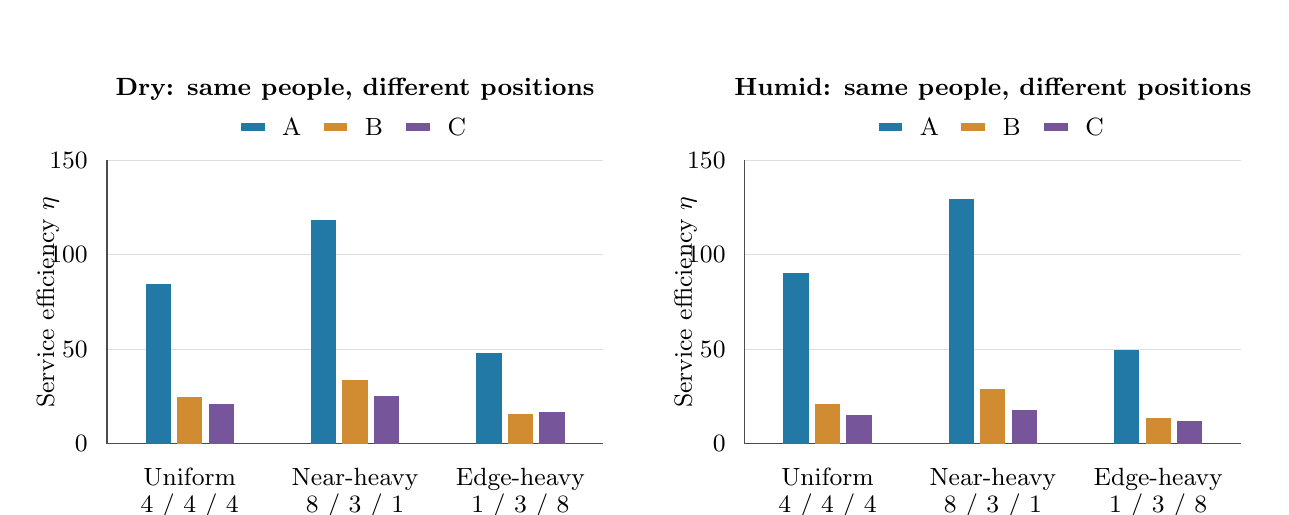
\begin{tikzpicture}[x=1cm,y=1cm,font=\fontsize{9}{10}\selectfont]
\definecolor{busA}{HTML}{2379A5}
\definecolor{busB}{HTML}{D18C32}
\definecolor{busC}{HTML}{76559A}
\begin{scope}[xshift=0.0cm]
\draw[black!13] (0.0000,0.0000) -- (6.3000,0.0000);
\node[anchor=east] at (-0.1200,0.0000) {0};
\draw[black!13] (0.0000,1.2000) -- (6.3000,1.2000);
\node[anchor=east] at (-0.1200,1.2000) {50};
\draw[black!13] (0.0000,2.4000) -- (6.3000,2.4000);
\node[anchor=east] at (-0.1200,2.4000) {100};
\draw[black!13] (0.0000,3.6000) -- (6.3000,3.6000);
\node[anchor=east] at (-0.1200,3.6000) {150};
\draw[black!70] (0.0000,0.0000) -- (6.3000,0.0000);
\draw[black!70] (0.0000,0.0000) -- (0.0000,3.6000);
\node[align=center] at (3.1500,4.5000) {\textbf{Dry: same people, different positions}};
\node[rotate=90,align=center] at (-0.7500,1.8000) {Service efficiency $\eta$};
\draw[busA,line width=3pt] (1.7000,4.0200) -- (2.0000,4.0200);
\node[anchor=west] at (2.1000,4.0200) {A};
\draw[busB,line width=3pt] (2.7500,4.0200) -- (3.0500,4.0200);
\node[anchor=west] at (3.1500,4.0200) {B};
\draw[busC,line width=3pt] (3.8000,4.0200) -- (4.1000,4.0200);
\node[anchor=west] at (4.2000,4.0200) {C};
\fill[busA] (0.4900,0) rectangle (0.8100,2.0298);
\fill[busB] (0.8900,0) rectangle (1.2100,0.5883);
\fill[busC] (1.2900,0) rectangle (1.6100,0.5073);
\node[align=center,anchor=north] at (1.0500,-0.1800) {Uniform\\4 / 4 / 4};
\fill[busA] (2.5900,0) rectangle (2.9100,2.8402);
\fill[busB] (2.9900,0) rectangle (3.3100,0.8043);
\fill[busC] (3.3900,0) rectangle (3.7100,0.6089);
\node[align=center,anchor=north] at (3.1500,-0.1800) {Near-heavy\\8 / 3 / 1};
\fill[busA] (4.6900,0) rectangle (5.0100,1.1586);
\fill[busB] (5.0900,0) rectangle (5.4100,0.3726);
\fill[busC] (5.4900,0) rectangle (5.8100,0.3992);
\node[align=center,anchor=north] at (5.2500,-0.1800) {Edge-heavy\\1 / 3 / 8};
\end{scope}
\begin{scope}[xshift=8.1cm]
\draw[black!13] (0.0000,0.0000) -- (6.3000,0.0000);
\node[anchor=east] at (-0.1200,0.0000) {0};
\draw[black!13] (0.0000,1.2000) -- (6.3000,1.2000);
\node[anchor=east] at (-0.1200,1.2000) {50};
\draw[black!13] (0.0000,2.4000) -- (6.3000,2.4000);
\node[anchor=east] at (-0.1200,2.4000) {100};
\draw[black!13] (0.0000,3.6000) -- (6.3000,3.6000);
\node[anchor=east] at (-0.1200,3.6000) {150};
\draw[black!70] (0.0000,0.0000) -- (6.3000,0.0000);
\draw[black!70] (0.0000,0.0000) -- (0.0000,3.6000);
\node[align=center] at (3.1500,4.5000) {\textbf{Humid: same people, different positions}};
\node[rotate=90,align=center] at (-0.7500,1.8000) {Service efficiency $\eta$};
\draw[busA,line width=3pt] (1.7000,4.0200) -- (2.0000,4.0200);
\node[anchor=west] at (2.1000,4.0200) {A};
\draw[busB,line width=3pt] (2.7500,4.0200) -- (3.0500,4.0200);
\node[anchor=west] at (3.1500,4.0200) {B};
\draw[busC,line width=3pt] (3.8000,4.0200) -- (4.1000,4.0200);
\node[anchor=west] at (4.2000,4.0200) {C};
\fill[busA] (0.4900,0) rectangle (0.8100,2.1736);
\fill[busB] (0.8900,0) rectangle (1.2100,0.5068);
\fill[busC] (1.2900,0) rectangle (1.6100,0.3641);
\node[align=center,anchor=north] at (1.0500,-0.1800) {Uniform\\4 / 4 / 4};
\fill[busA] (2.5900,0) rectangle (2.9100,3.1027);
\fill[busB] (2.9900,0) rectangle (3.3100,0.6920);
\fill[busC] (3.3900,0) rectangle (3.7100,0.4287);
\node[align=center,anchor=north] at (3.1500,-0.1800) {Near-heavy\\8 / 3 / 1};
\fill[busA] (4.6900,0) rectangle (5.0100,1.1972);
\fill[busB] (5.0900,0) rectangle (5.4100,0.3233);
\fill[busC] (5.4900,0) rectangle (5.8100,0.2937);
\node[align=center,anchor=north] at (5.2500,-0.1800) {Edge-heavy\\1 / 3 / 8};
\end{scope}
\end{tikzpicture}

\caption{Moving the same 12 mean occupants between near, middle, and edge zones changes delivered service. Labels give the three zone occupancies.}
\label{fig:bus-occupancy}
\end{figure}

In dry conditions, A's efficiency falls from $118.3$ under near-heavy occupancy to $48.3$ under edge-heavy occupancy. More importantly, the B/C ordering reverses: under uniform occupancy B exceeds C ($24.5$ versus $21.1$), while at the edge-heavy stop C exceeds B ($16.6$ versus $15.5$). The same total population is being served; the change comes from where people stand relative to the assumed delivery fields. A remains the most energy-efficient option in all six nominal climate--occupancy cases.

\clearpage
\subsection{When the recommendation changes}

A poorly aimed or obstructed fan can consume electricity without delivering its nominal air movement to passengers. We test this specific failure mode using
\begin{equation}
 v_{A,z}(q)=v_0+q(v_{A,z}^{\mathrm{nom}}-v_0),\qquad 0\leq q\leq1,
\end{equation}
while holding $P_A=0.25$ kW. Here $q$ describes delivery loss at occupied positions, \emph{not} a fan-speed control setting; changing motor speed would require a different power model. The B/C profiles stay fixed in this particular stress test.

\begin{figure}[!ht]
\centering
% Fully embedded Figure 05; only the standard tikz package is required.
% Source: fan_delivery_thresholds.csv and delivery_decision_map.csv.
% RH columns: 20--80 percent in 1 percentage-point steps; q step: 0.02.
% The white line is the first A-winning grid q. The colored cell boundary
% lies 0.01 below it, as in the nearest-grid-cell rendering of the PNG.
% All data are embedded below: no external graphics, CSV, input, or shell escape.
\begingroup
\definecolor{businlineA}{HTML}{2379A5}
\definecolor{businlineB}{HTML}{D18C32}
\definecolor{businlineC}{HTML}{76559A}
\begin{tikzpicture}[x=0.16cm,y=4.5cm,
  font=\fontsize{9.5pt}{11pt}\selectfont,
  every node/.style={inner sep=1.5pt},line width=0.5pt]
% Plot size 9.6 cm by 4.5 cm; complete drawing remains below 15 cm by 7 cm.
\path[fill=businlineA,draw=none] (20,0) rectangle (80,1);
\path[fill=businlineB,draw=none] (20.0,0) rectangle (58.5,0.17);
\path[fill=businlineB,draw=none] (58.5,0) rectangle (73.5,0.15);
\path[fill=businlineB,draw=none] (73.5,0) rectangle (80.0,0.13);

% Reference grid and observed grid-resolved transition.
\foreach \q in {0.2,0.4,0.6,0.8}
  \draw[white,opacity=0.16,line width=0.3pt] (20,\q) -- (80,\q);
\draw[white,line width=1.05pt,line join=round] (20,0.18) --
  (21,0.18) --
  (22,0.18) --
  (23,0.18) --
  (24,0.18) --
  (25,0.18) --
  (26,0.18) --
  (27,0.18) --
  (28,0.18) --
  (29,0.18) --
  (30,0.18) --
  (31,0.18) --
  (32,0.18) --
  (33,0.18) --
  (34,0.18) --
  (35,0.18) --
  (36,0.18) --
  (37,0.18) --
  (38,0.18) --
  (39,0.18) --
  (40,0.18) --
  (41,0.18) --
  (42,0.18) --
  (43,0.18) --
  (44,0.18) --
  (45,0.18) --
  (46,0.18) --
  (47,0.18) --
  (48,0.18) --
  (49,0.18) --
  (50,0.18) --
  (51,0.18) --
  (52,0.18) --
  (53,0.18) --
  (54,0.18) --
  (55,0.18) --
  (56,0.18) --
  (57,0.18) --
  (58,0.18) --
  (59,0.16) --
  (60,0.16) --
  (61,0.16) --
  (62,0.16) --
  (63,0.16) --
  (64,0.16) --
  (65,0.16) --
  (66,0.16) --
  (67,0.16) --
  (68,0.16) --
  (69,0.16) --
  (70,0.16) --
  (71,0.16) --
  (72,0.16) --
  (73,0.16) --
  (74,0.14) --
  (75,0.14) --
  (76,0.14) --
  (77,0.14) --
  (78,0.14) --
  (79,0.14) --
  (80,0.14);
\draw[black] (20,0) rectangle (80,1);

% Tick marks are given in physical units so they remain equal in length.
\foreach \x in {20,30,40,50,60,70,80}{
  \draw (\x,0) -- ++(0,-0.022);
  \node[anchor=north] at (\x,-0.027) {\x};
}
\foreach \q/\lab in {0/0.0,0.2/0.2,0.4/0.4,0.6/0.6,0.8/0.8,1/1.0}{
  \draw (20,\q) -- ++(-0.62,0);
  \node[anchor=east] at (19.2,\q) {\lab};
}
\node[anchor=north] at (50,-0.108) {Ambient relative humidity (\%)};
\node[rotate=90] at (13.5,0.5) {Fan air-speed delivery fraction $q$};
\node[anchor=south,font=\fontsize{10pt}{12pt}\selectfont]
  at (50,1.045) {Highest service efficiency under fan delivery loss};

% Two definitions inside the plotting area, as in the original figure.
\node[white,anchor=north east] at (78.8,0.948)
  {$q=1$: nominal fan profile.};
\node[white,anchor=north east] at (78.8,0.875)
  {$q=0$: no added air speed at occupied positions.};

% C remains a considered alternative, but wins no cells on this grid.
\path[fill=businlineA] (82.5,0.825) rectangle (84.1,0.879);
\node[anchor=west] at (85.1,0.852) {A: fan};
\path[fill=businlineB] (82.5,0.705) rectangle (84.1,0.759);
\node[anchor=west] at (85.1,0.732) {B: evaporative};
\path[fill=businlineC] (82.5,0.585) rectangle (84.1,0.639);
\node[anchor=west,align=left] at (85.1,0.612) {C: no winning cells};
\node[anchor=north west,align=left,text width=2.85cm] at (82.4,0.445)
  {White line: first\\A-winning grid $q$.};
\node[anchor=north west,align=left,text width=2.85cm] at (82.4,0.265)
  {Grid spacing:\\RH: 1 percentage point;\\$q$: 0.02.};
\end{tikzpicture}
\endgroup

\caption{Conditional efficiency winner on the complete RH--fan-delivery grid: RH $20$--$80\%$ in one-percentage-point steps and $q=0$--$1$ in steps of $0.02$. The boundary is grid-resolved. This tests fan delivery loss; it is not a universal climate-selection map.}
\label{fig:bus-decision}
\end{figure}

The first sampled $q$ at which A wins is $0.18$ at RH $30\%$ and $0.16$ at RH $70\%$; the corresponding switch lies between that sample and the preceding $0.02$ grid step. At lower delivery, B wins. C has no winning cells in this particular grid, although it provides greater absolute relief in the nominal cases. Every humidity column has one contiguous A-winning interval. These boundaries depend on the prescribed B/C fields and are not real-world probabilities or universal fan-performance thresholds.

\noindent\textbf{Operational interpretation.} First preserve shade and place people within useful airflow. Compare the measured benefit of improving equipment placement with the benefit of adding cooling capacity. If a larger evaporative system serves substantially more occupied space, use Eq.~\eqref{eq:break-even} with its measured service to decide whether that expansion compensates for electricity use. In humid conditions, an assumed larger nominal temperature drop cannot override the wet-bulb constraint.

A field calibration would measure $(T,\mathrm{RH},v,T_r)$ at occupied positions, electricity over the same period, and occupancy by zone. Repeated matched weather and occupancy conditions would allow the assumed profiles in Table~\ref{tab:bus-fields} to be replaced and the ranking checked. The quoted $3/5/8\,^{\circ}\mathrm C$ effects alone cannot supply this calibration.

\clearpage
\subsection{Sensitivity, verification, and scope}

\begin{figure}[!ht]
\centering
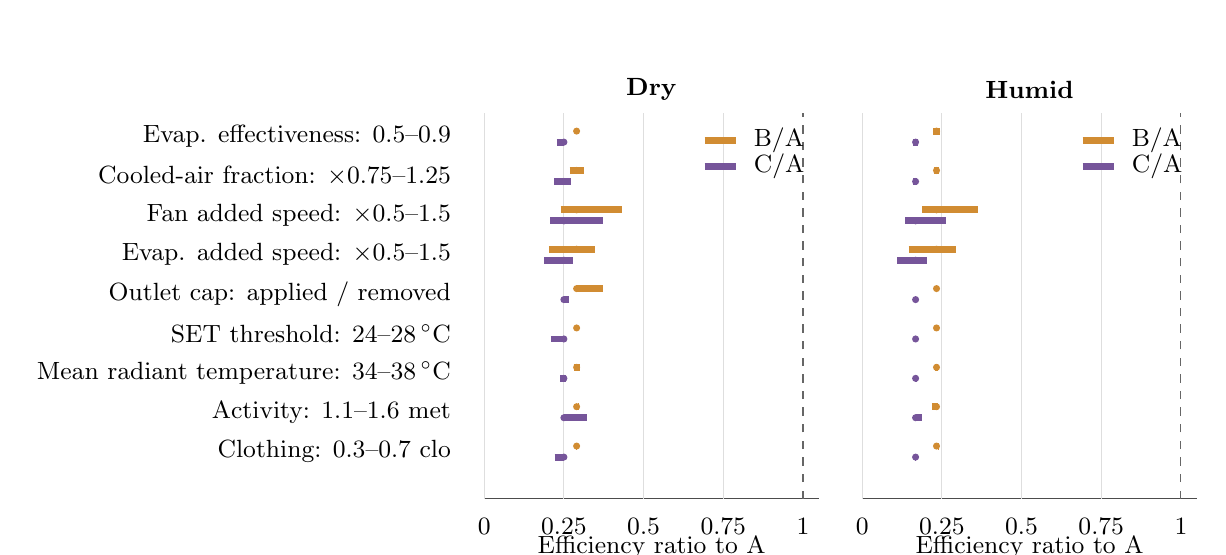
\begin{tikzpicture}[x=1cm,y=1cm,font=\fontsize{9}{10}\selectfont]
\definecolor{busA}{HTML}{2379A5}
\definecolor{busB}{HTML}{D18C32}
\definecolor{busC}{HTML}{76559A}
\node[anchor=east] at (5.5000,4.6000) {Evap. effectiveness: $0.5$--$0.9$};
\node[anchor=east] at (5.5000,4.1000) {Cooled-air fraction: $\times0.75$--$1.25$};
\node[anchor=east] at (5.5000,3.6000) {Fan added speed: $\times0.5$--$1.5$};
\node[anchor=east] at (5.5000,3.1000) {Evap. added speed: $\times0.5$--$1.5$};
\node[anchor=east] at (5.5000,2.6000) {Outlet cap: applied / removed};
\node[anchor=east] at (5.5000,2.1000) {SET threshold: $24$--$28\,^{\circ}$C};
\node[anchor=east] at (5.5000,1.6000) {Mean radiant temperature: $34$--$38\,^{\circ}$C};
\node[anchor=east] at (5.5000,1.1000) {Activity: $1.1$--$1.6$ met};
\node[anchor=east] at (5.5000,0.6000) {Clothing: $0.3$--$0.7$ clo};
\node[] at (7.9250,5.2000) {\textbf{Dry}};
\draw[black!70] (5.8000,0.0000) -- (10.0500,0.0000);
\draw[black!13] (5.8000,0.0000) -- (5.8000,4.9000);
\node[anchor=north] at (5.8000,-0.1200) {0};
\draw[black!13] (6.8119,0.0000) -- (6.8119,4.9000);
\node[anchor=north] at (6.8119,-0.1200) {0.25};
\draw[black!13] (7.8238,0.0000) -- (7.8238,4.9000);
\node[anchor=north] at (7.8238,-0.1200) {0.5};
\draw[black!13] (8.8357,0.0000) -- (8.8357,4.9000);
\node[anchor=north] at (8.8357,-0.1200) {0.75};
\draw[black!60,dashed] (9.8476,0.0000) -- (9.8476,4.9000);
\node[anchor=north] at (9.8476,-0.1200) {1};
\draw[busB,line width=2.5pt] (6.9730,4.6700) -- (6.9730,4.6700);
\fill[busB] (6.9730,4.6700) circle (0.045);
\draw[busC,line width=2.5pt] (6.7238,4.5300) -- (6.8115,4.5300);
\fill[busC] (6.8115,4.5300) circle (0.045);
\draw[busB,line width=2.5pt] (6.8830,4.1700) -- (7.0658,4.1700);
\fill[busB] (6.9730,4.1700) circle (0.045);
\draw[busC,line width=2.5pt] (6.6884,4.0300) -- (6.8993,4.0300);
\fill[busC] (6.8115,4.0300) circle (0.045);
\draw[busB,line width=2.5pt] (6.7695,3.6700) -- (7.5473,3.6700);
\fill[busB] (6.9730,3.6700) circle (0.045);
\draw[busC,line width=2.5pt] (6.6361,3.5300) -- (7.3068,3.5300);
\fill[busC] (6.8115,3.5300) circle (0.045);
\draw[busB,line width=2.5pt] (6.6208,3.1700) -- (7.2082,3.1700);
\fill[busB] (6.9730,3.1700) circle (0.045);
\draw[busC,line width=2.5pt] (6.5617,3.0300) -- (6.9319,3.0300);
\fill[busC] (6.8115,3.0300) circle (0.045);
\draw[busB,line width=2.5pt] (6.9730,2.6700) -- (7.3019,2.6700);
\fill[busB] (6.9730,2.6700) circle (0.045);
\draw[busC,line width=2.5pt] (6.8115,2.5300) -- (6.8747,2.5300);
\fill[busC] (6.8115,2.5300) circle (0.045);
\draw[busB,line width=2.5pt] (6.9730,2.1700) -- (6.9730,2.1700);
\fill[busB] (6.9730,2.1700) circle (0.045);
\draw[busC,line width=2.5pt] (6.6472,2.0300) -- (6.8115,2.0300);
\fill[busC] (6.8115,2.0300) circle (0.045);
\draw[busB,line width=2.5pt] (6.9338,1.6700) -- (7.0207,1.6700);
\fill[busB] (6.9730,1.6700) circle (0.045);
\draw[busC,line width=2.5pt] (6.7652,1.5300) -- (6.8422,1.5300);
\fill[busC] (6.8115,1.5300) circle (0.045);
\draw[busB,line width=2.5pt] (6.9851,1.1700) -- (7.0049,1.1700);
\fill[busB] (6.9730,1.1700) circle (0.045);
\draw[busC,line width=2.5pt] (6.8123,1.0300) -- (7.1089,1.0300);
\fill[busC] (6.8115,1.0300) circle (0.045);
\draw[busB,line width=2.5pt] (6.9677,0.6700) -- (6.9727,0.6700);
\fill[busB] (6.9730,0.6700) circle (0.045);
\draw[busC,line width=2.5pt] (6.6933,0.5300) -- (6.8145,0.5300);
\fill[busC] (6.8115,0.5300) circle (0.045);
\node[] at (7.9250,-0.6200) {Efficiency ratio to A};
\draw[busB,line width=2.5pt] (8.6000,4.5500) -- (9.0000,4.5500);
\node[anchor=west] at (9.1000,4.5500) {B/A};
\draw[busC,line width=2.5pt] (8.6000,4.2200) -- (9.0000,4.2200);
\node[anchor=west] at (9.1000,4.2200) {C/A};
\node[] at (12.7250,5.2000) {\textbf{Humid}};
\draw[black!70] (10.6000,0.0000) -- (14.8500,0.0000);
\draw[black!13] (10.6000,0.0000) -- (10.6000,4.9000);
\node[anchor=north] at (10.6000,-0.1200) {0};
\draw[black!13] (11.6119,0.0000) -- (11.6119,4.9000);
\node[anchor=north] at (11.6119,-0.1200) {0.25};
\draw[black!13] (12.6238,0.0000) -- (12.6238,4.9000);
\node[anchor=north] at (12.6238,-0.1200) {0.5};
\draw[black!13] (13.6357,0.0000) -- (13.6357,4.9000);
\node[anchor=north] at (13.6357,-0.1200) {0.75};
\draw[black!60,dashed] (14.6476,0.0000) -- (14.6476,4.9000);
\node[anchor=north] at (14.6476,-0.1200) {1};
\draw[busB,line width=2.5pt] (11.5041,4.6700) -- (11.5843,4.6700);
\fill[busB] (11.5437,4.6700) circle (0.045);
\draw[busC,line width=2.5pt] (11.2440,4.5300) -- (11.3130,4.5300);
\fill[busC] (11.2780,4.5300) circle (0.045);
\draw[busB,line width=2.5pt] (11.5091,4.1700) -- (11.5790,4.1700);
\fill[busB] (11.5437,4.1700) circle (0.045);
\draw[busC,line width=2.5pt] (11.2482,4.0300) -- (11.2993,4.0300);
\fill[busC] (11.2780,4.0300) circle (0.045);
\draw[busB,line width=2.5pt] (11.3626,3.6700) -- (12.0724,3.6700);
\fill[busB] (11.5437,3.6700) circle (0.045);
\draw[busC,line width=2.5pt] (11.1478,3.5300) -- (11.6578,3.5300);
\fill[busC] (11.2780,3.5300) circle (0.045);
\draw[busB,line width=2.5pt] (11.1890,3.1700) -- (11.7933,3.1700);
\fill[busB] (11.5437,3.1700) circle (0.045);
\draw[busC,line width=2.5pt] (11.0480,3.0300) -- (11.4274,3.0300);
\fill[busC] (11.2780,3.0300) circle (0.045);
\draw[busB,line width=2.5pt] (11.5437,2.6700) -- (11.5437,2.6700);
\fill[busB] (11.5437,2.6700) circle (0.045);
\draw[busC,line width=2.5pt] (11.2780,2.5300) -- (11.2780,2.5300);
\fill[busC] (11.2780,2.5300) circle (0.045);
\draw[busB,line width=2.5pt] (11.5437,2.1700) -- (11.5437,2.1700);
\fill[busB] (11.5437,2.1700) circle (0.045);
\draw[busC,line width=2.5pt] (11.2780,2.0300) -- (11.2780,2.0300);
\fill[busC] (11.2780,2.0300) circle (0.045);
\draw[busB,line width=2.5pt] (11.5294,1.6700) -- (11.5629,1.6700);
\fill[busB] (11.5437,1.6700) circle (0.045);
\draw[busC,line width=2.5pt] (11.2651,1.5300) -- (11.2933,1.5300);
\fill[busC] (11.2780,1.5300) circle (0.045);
\draw[busB,line width=2.5pt] (11.4855,1.1700) -- (11.5577,1.1700);
\fill[busB] (11.5437,1.1700) circle (0.045);
\draw[busC,line width=2.5pt] (11.2784,1.0300) -- (11.3644,1.0300);
\fill[busC] (11.2780,1.0300) circle (0.045);
\draw[busB,line width=2.5pt] (11.5572,0.6700) -- (11.5578,0.6700);
\fill[busB] (11.5437,0.6700) circle (0.045);
\draw[busC,line width=2.5pt] (11.2727,0.5300) -- (11.2779,0.5300);
\fill[busC] (11.2780,0.5300) circle (0.045);
\node[] at (12.7250,-0.6200) {Efficiency ratio to A};
\draw[busB,line width=2.5pt] (13.4000,4.5500) -- (13.8000,4.5500);
\node[anchor=west] at (13.9000,4.5500) {B/A};
\draw[busC,line width=2.5pt] (13.4000,4.2200) -- (13.8000,4.2200);
\node[anchor=west] at (13.9000,4.2200) {C/A};
\end{tikzpicture}

\caption{One-factor-at-a-time sensitivity at the two endpoint settings listed on each row; dots mark nominal ratios. An interval above one would favor the evaporative device over A. These are assumed parameter ranges, not statistical confidence intervals. Joint uncertainty can produce changes beyond these endpoint tests.}
\label{fig:bus-sensitivity}
\end{figure}

Across the tested individual endpoint changes, the largest B/A and C/A efficiency ratios are $0.432$ and $0.372$; no endpoint reverses the nominal advantage of A. This does not prove robustness over every intermediate value or joint parameter combination. Added-speed factors scale $v-v_0$, and cooled-air fractions are capped at one. The rating-interpretation test removes the $5/8\,^{\circ}\mathrm C$ outlet caps while retaining the wet-bulb constraint; it addresses uncertainty in where the quoted temperature effects were measured. The delivery-loss test in Figure~\ref{fig:bus-decision} already demonstrates that stronger departures can change the winner.

\noindent\textbf{Verification.} The implementation checks psychrometric round trips, dry-air moisture/enthalpy mixing balances, wet-bulb bounds, and saturation. Service-accounting checks verify $U_s+R_s=R_0$, zero benefit at zero occupancy, zero benefit when all delivered effects vanish, and unchanged rankings when every zone's population doubles. A signed-adverse-effect check confirms that worsening discomfort is not clipped away. No credit is given for additional cooling of an already comfortable baseline.

\noindent\textbf{Limitations and transfer.} Local profiles and representative passengers remain assumptions; the numerical ranking is conditional on them. Airflow and dilution are prescribed rather than solved from fan curves, mass flow, crosswind, and shelter geometry. Radiation is fixed for a shaded shelter, so direct sun and changing shadow patterns need additional modeling. Short waiting times and varied physiological histories are not resolved by quasi-steady SET. Without measured flow, water consumption cannot be calculated reliably from the moisture increase alone; water and operating cost belong in the later effectiveness analysis. For a semi-open station, the same service accounting can be retained while adding enclosure heat storage and air/moisture exchange to the environment model.

\noindent\textbf{Reproducibility.} Calculations use \texttt{pythermalcomfort} 4.8.1 and PsychroLib 2.5.0. The accompanying \texttt{bus\_model} folder contains the scenario parameters, psychrometric/SET backend, executable simulation, CSV outputs, source audit, and all six figures. The figures are also embedded as vector drawings in this source file. Software versions and checks are saved with the results. Simulations quantify the stated assumptions; they do not constitute experimental validation.

\clearpage
\phantomsection
\addcontentsline{toc}{section}{References}
\begin{thebibliography}{99}
\bibitem{ashrae}
ASHRAE. \emph{2026 ASHRAE Handbook---Refrigeration},
Chapter 15, \emph{Retail Food Store Refrigeration and Equipment}.
Product Temperatures and Display Refrigerator Cooling Load sections.
\url{https://handbook.ashrae.org/Handbooks/R26/IP/r26_ch15/r26_ch15_ip.aspx}.
Accessed November 7, 2026.

\bibitem{etl}
UK Department for Energy Security and Net Zero.
\emph{Energy Technology List: Retrofit Measures for Open Fronted Refrigerated Display Cabinets}.
Definitions and product-temperature performance requirements.
\url{https://etl.energysecurity.gov.uk/products/refrigeration-equipment/retrofit-measures-open-fronted-refrigerated-display-cabinets}.
Accessed November 7, 2026.

\bibitem{energystar}
ENERGY STAR. \emph{Ceiling Fan Installation and Usage Tips}.
\url{https://www.energystar.gov/products/ceiling_fans/installation-and-usage-tips}.
Accessed November 7, 2026.

\bibitem{evap}
ASHRAE. \emph{2023 ASHRAE Handbook---HVAC Applications},
Chapter 53, \emph{Evaporative Cooling}.
\url{https://handbook.ashrae.org/Handbooks/A23/SI/A23_Ch53/a23_ch53_si.aspx}.
Accessed November 7, 2026.

\bibitem{problem}
COMAP. \emph{2026 HiMCM Problem B: Air Conditioning the Environment: Modeling Energy Waste in Public Cooling}.
User-supplied problem statement, Requirement 2(a), p.~2.

\bibitem{evapequip}
ASHRAE. \emph{2020 ASHRAE Handbook---HVAC Systems and Equipment},
Chapter 41, \emph{Evaporative Air-Cooling Equipment}, Section 1.
\url{https://handbook.ashrae.org/handbooks/S20/SI/s20_ch41/s20_ch41_si.aspx}.
Accessed November 7, 2026.

\bibitem{fanguide}
Center for the Built Environment, University of California, Berkeley.
\emph{Fans for Cooling People Guidebook: Elevated Air Speed and Thermal Comfort}.
\url{https://cbe-berkeley.gitbook.io/fans-guidebook/full-guidebook/elevated-air-speed-and-thermal-comfort}.
Accessed November 7, 2026.

\bibitem{thermalcomfort}
ASHRAE. \emph{2017 ASHRAE Handbook---Fundamentals},
Chapter 9, \emph{Thermal Comfort}, Section 10, Environmental Indices.
\url{https://handbook.ashrae.org/Handbooks/f17/IP/f17_ch09/f17_ch09_ip.aspx}.
Accessed November 7, 2026.

\bibitem{pythermal}
Tartarini, F., and Schiavon, S. (2020).
pythermalcomfort: A Python package for thermal comfort research.
\emph{SoftwareX}, 12, 100578.
\url{https://doi.org/10.1016/j.softx.2020.100578}.
SET API and applicability limits:
\url{https://pythermalcomfort.readthedocs.io/en/stable/documentation/models.html}.
Accessed November 7, 2026.

\bibitem{psychrolib}
Meyer, D., and Thevenard, D. (2019).
PsychroLib: a library of psychrometric functions to calculate thermodynamic properties of air.
\emph{Journal of Open Source Software}, 4(33), 1137.
\url{https://doi.org/10.21105/joss.01137}.
SI psychrometric API:
\url{https://psychrometrics.github.io/psychrolib/api_docs.html}.
Accessed November 7, 2026.

\bibitem{gemini}
Google Gemini. \emph{AI-generated analysis of the 2026 HiMCM Problem B},
user-supplied PDF conversation excerpt, November 2026.
Consulted for process-oriented exposition; the proposed efficiency formula was
reviewed but not adopted. Exact model identifier was not available in the supplied excerpt.

\bibitem{codex}
OpenAI. \emph{Codex}, AI-assisted formulation, reference checking,
English drafting, and LaTeX preparation, November 2026.
Exact deployed model identifier to be recorded from the session interface.
See the preliminary AI-use record following this draft.

\bibitem{aipolicy}
COMAP. \emph{Use of AI Tools in COMAP Contests}, v102025.
\url{https://www.contest.comap.com/undergraduate/contests/mcm/flyer/Contest_AI_Policy.pdf}.
Accessed November 7, 2026.
\end{thebibliography}

% Add Requirement 2(b), Requirements 3--5, the memorandum, and the blog before References.
% Replace the working summary after completing the full analysis.
\clearpage
\phantomsection
\addcontentsline{toc}{section}{Report on Use of AI Tools}
\section*{Report on Use of AI Tools}
\noindent\textbf{Preliminary record for this partial draft.}

OpenAI Codex assisted with problem translation, the overall modeling discussion,
and the development of Requirements 1 and 2(a) in November 2026. The exact deployed model
identifier must be recorded from the session interface.

For this edit, the user requested an English section in the supplied template
covering infiltration, cabinet heat transfer, internal equipment, restocking,
defrost and operating cycles, equipment age, and spatial temperatures. This is
a summary of the request, not a verbatim transcript.

The assistant proposed and subsequently simplified the evaluation framework,
checked source material, drafted the English text, and prepared the LaTeX.
Separate AI review passes checked technical consistency. At the user's request,
the 2025 Problem B solutions of Teams 16442, 16738, and 16739 were reviewed as
structural references. Their numerical estimates, weighting procedures, and
wording were not used in the present model. This revision emphasizes indicator
justification and transfer to the later task. No field measurements or empirical
performance results were produced.

A user-supplied Google Gemini conversation excerpt was subsequently reviewed.
Its process-oriented explanation informed the organization of the new diagram;
Codex redrew and revised the dependencies and service definitions. The Gemini
model identifier and complete conversation were not available in that excerpt.
The relevant Gemini prompts and outputs must also be included in the final record.

For Requirement 2(a), the user authorized development of the bus-stop extension,
requested explicit citations, and asked for multiple charts. Codex formulated the
three-zone scenario, wrote Python code, used PsychroLib and pythermalcomfort for
psychrometric and SET calculations, generated six figures and CSV results, and
drafted the accompanying interpretation. AI review passes checked the physical
assumptions, source support, and correspondence between equations and code.
The numerical checks establish internal consistency; no field validation is
claimed. Unmeasured delivery profiles are explicitly labeled assumptions.
Software versions are recorded in the accompanying results file. The full
relevant prompts, outputs, and code-generation record must be preserved in the
final AI-use report; this paragraph is only a summary of those contributions.

Before submission, add the exact relevant prompts and complete outputs,
including earlier retained contributions and any additional AI tools, as
required by the contest reporting guidance \cite{aipolicy}. Retain this source
file and the chat as records. The student team's independent verification is
still required and has not been asserted in this preliminary record.

\end{document}

